\documentclass[12pt]{article}
\usepackage{graphicx}
\usepackage{adjustbox}
\usepackage{amsmath}
\usepackage{amssymb}
\usepackage{hyperref}
\usepackage{fancyhdr}
\usepackage{cite}
\usepackage{geometry}
\usepackage{float}
\usepackage{caption}
\usepackage{siunitx}
\usepackage{pdfpages}
\usepackage{pdfpages}
\usepackage{listings}
\usepackage{xcolor}
\usepackage{subcaption}

\geometry{a4paper, margin=1in, top=1in, bottom=1in, left=1in, right=1in}

\definecolor{codeblue}{rgb}{0.0, 0.0, 0.6}
\definecolor{codegreen}{rgb}{0.0, 0.5, 0.0}
\definecolor{codegray}{rgb}{0.5, 0.5, 0.5}
\definecolor{codeorange}{rgb}{0.8, 0.4, 0.0}
\definecolor{backcolor}{rgb}{0.97, 0.97, 0.97}

\lstdefinestyle{python}{
    language=Python,
    backgroundcolor=\color{backcolor},
    basicstyle=\ttfamily\footnotesize,
    keywordstyle=\color{codeblue}\bfseries,
    commentstyle=\color{codegray}\itshape,
    stringstyle=\color{codegreen},
    numberstyle=\tiny\color{codegray},
    morekeywords=[2]{np, plt, solve_ivp, arange, exp, sin, cos, zeros_like,
                      array, imag, real, abs, max, savefig, subplot, subplots,
                      plot, stem, xlabel, ylabel, legend, grid, tight_layout,
                      figure, gradient, linspace, zeros},
    keywordstyle=[2]\color{codeorange},
    numbers=left,
    numbersep=8pt,
    breaklines=true,
    breakatwhitespace=false,
    showstringspaces=false,
    frame=single,
    rulecolor=\color{codegray},
    tabsize=4,
    captionpos=b,
    xleftmargin=1.5em,
    framexleftmargin=1.5em
}

\pagestyle{fancy}
\fancyhf{}
\fancyhead[L]{Signals Lab 2}
\fancyfoot[C]{\thepage}

\title{\textbf{Signals Lab 2 - Impulse Response, Step Response, and RC Circuits}}
\author{Colden Briggs - Eben Radocchia - Liam Donlan\\Instructor: Dr. Ossareh\\ University of Vermont}

\begin{document}

\maketitle
\newpage
\tableofcontents
\newpage

%---------------------------------------------------------------------
\section*{Introduction}
\addcontentsline{toc}{section}{Introduction}
% Objectives only 
%---------------------------------------------------------------------
\newpage
\section*{Task 1: Prelab Derivations}
\addcontentsline{toc}{section}{Task 1: Prelab Derivations}

\subsection*{1. Time constants and gain}
\addcontentsline{toc}{subsection}{Time constants and gain}
\begin{align*}
\tau_1 &= R_1C_1 = (\SI{10}{\kilo\ohm})(\SI{1}{\micro\farad}) = \SI{1.0e-2}{\second} \\
\tau_2 &= R_2C_2 = (\SI{4.7}{\kilo\ohm})(\SI{1}{\micro\farad}) = \SI{4.7e-3}{\second} \\
G &= 1 + \frac{R_5}{R_4} = 1 + \frac{\SI{4.7}{\kilo\ohm}}{\SI{1}{\kilo\ohm}} = 5.7
\end{align*}

\subsection*{2. Second-order ODE for $v_{c2}(t)$}
\addcontentsline{toc}{subsection}{Second-order ODE}
The two stages are described by
\begin{align*}
\dot v_{c1}(t) &= \frac{1}{\tau_1}\big(v_{in}(t) - v_{c1}(t)\big), \\
\dot v_{c2}(t) &= \frac{1}{\tau_2}\big(G\,v_{c1}(t) - v_{c2}(t)\big).
\end{align*}
Differentiating the second equation and substituting $\dot v_{c1}$ from the first:
\begin{align*}
\ddot v_{c2}(t) &= \frac{G}{\tau_2}\dot v_{c1}(t) - \frac{1}{\tau_2}\dot v_{c2}(t) \\
&= \frac{G}{\tau_1\tau_2}\big(v_{in}(t) - v_{c1}(t)\big) - \frac{1}{\tau_2}\dot v_{c2}(t).
\end{align*}
Solving the second stage equation for $v_{c1}$ gives
\[
v_{c1}(t) = \frac{\tau_2\,\dot v_{c2}(t) + v_{c2}(t)}{G},
\]
and substituting this in:
\begin{align*}
\ddot v_{c2}(t) &= \frac{G}{\tau_1\tau_2}v_{in}(t) - \frac{1}{\tau_1\tau_2}\big(\tau_2\dot v_{c2}(t) + v_{c2}(t)\big) - \frac{1}{\tau_2}\dot v_{c2}(t) \\
&= \frac{G}{\tau_1\tau_2}v_{in}(t) - \frac{1}{\tau_1}\dot v_{c2}(t) - \frac{1}{\tau_1\tau_2}v_{c2}(t) - \frac{1}{\tau_2}\dot v_{c2}(t).
\end{align*}
Collecting terms:
\[
\boxed{\ddot v_{c2}(t) + \left(\frac{1}{\tau_1} + \frac{1}{\tau_2}\right)\dot v_{c2}(t) + \frac{1}{\tau_1\tau_2}v_{c2}(t) = \frac{G}{\tau_1\tau_2}v_{in}(t)}
\]

\subsection*{3. Impulse response $h(t)$}
\addcontentsline{toc}{subsection}{Impulse response}
For an impulse input, the first stage output is the single-stage RC impulse response (Section 1.1 with $\tau = \tau_1$):
\[
v_{c1}(t) = \frac{1}{\tau_1}e^{-t/\tau_1}u(t).
\]
Plugging this into the second stage ODE, for $t \ge 0$:
\[
\dot v_{c2}(t) + \frac{1}{\tau_2}v_{c2}(t) = \frac{G}{\tau_1\tau_2}e^{-t/\tau_1}.
\]
Using the integrating factor $\mu = e^{t/\tau_2}$:
\[
v_{c2}(t) = e^{-t/\tau_2}\left(\int \frac{G}{\tau_1\tau_2}\,e^{t/\tau_2 - t/\tau_1}\,dt + C\right).
\]
The exponent simplifies to
\[
\frac{t}{\tau_2} - \frac{t}{\tau_1} = \frac{t(\tau_1 - \tau_2)}{\tau_1\tau_2},
\]
so the integral is
\[
\int \frac{G}{\tau_1\tau_2}\,e^{\frac{t(\tau_1-\tau_2)}{\tau_1\tau_2}}\,dt = \frac{G}{\tau_1 - \tau_2}\,e^{\frac{t(\tau_1-\tau_2)}{\tau_1\tau_2}},
\]
which gives
\[
v_{c2}(t) = \frac{G}{\tau_1 - \tau_2}e^{-t/\tau_1} + C\,e^{-t/\tau_2}.
\]
The initial condition $v_{c2}(0) = 0$ gives $C = -\dfrac{G}{\tau_1 - \tau_2}$. Therefore
\[
\boxed{h(t) = \frac{G}{\tau_1 - \tau_2}\left(e^{-t/\tau_1} - e^{-t/\tau_2}\right)u(t)}
\]
Figure \ref{fig:h_analytic} shows $h(t)$ for the given component values.
\begin{figure}[H]
    \centering
     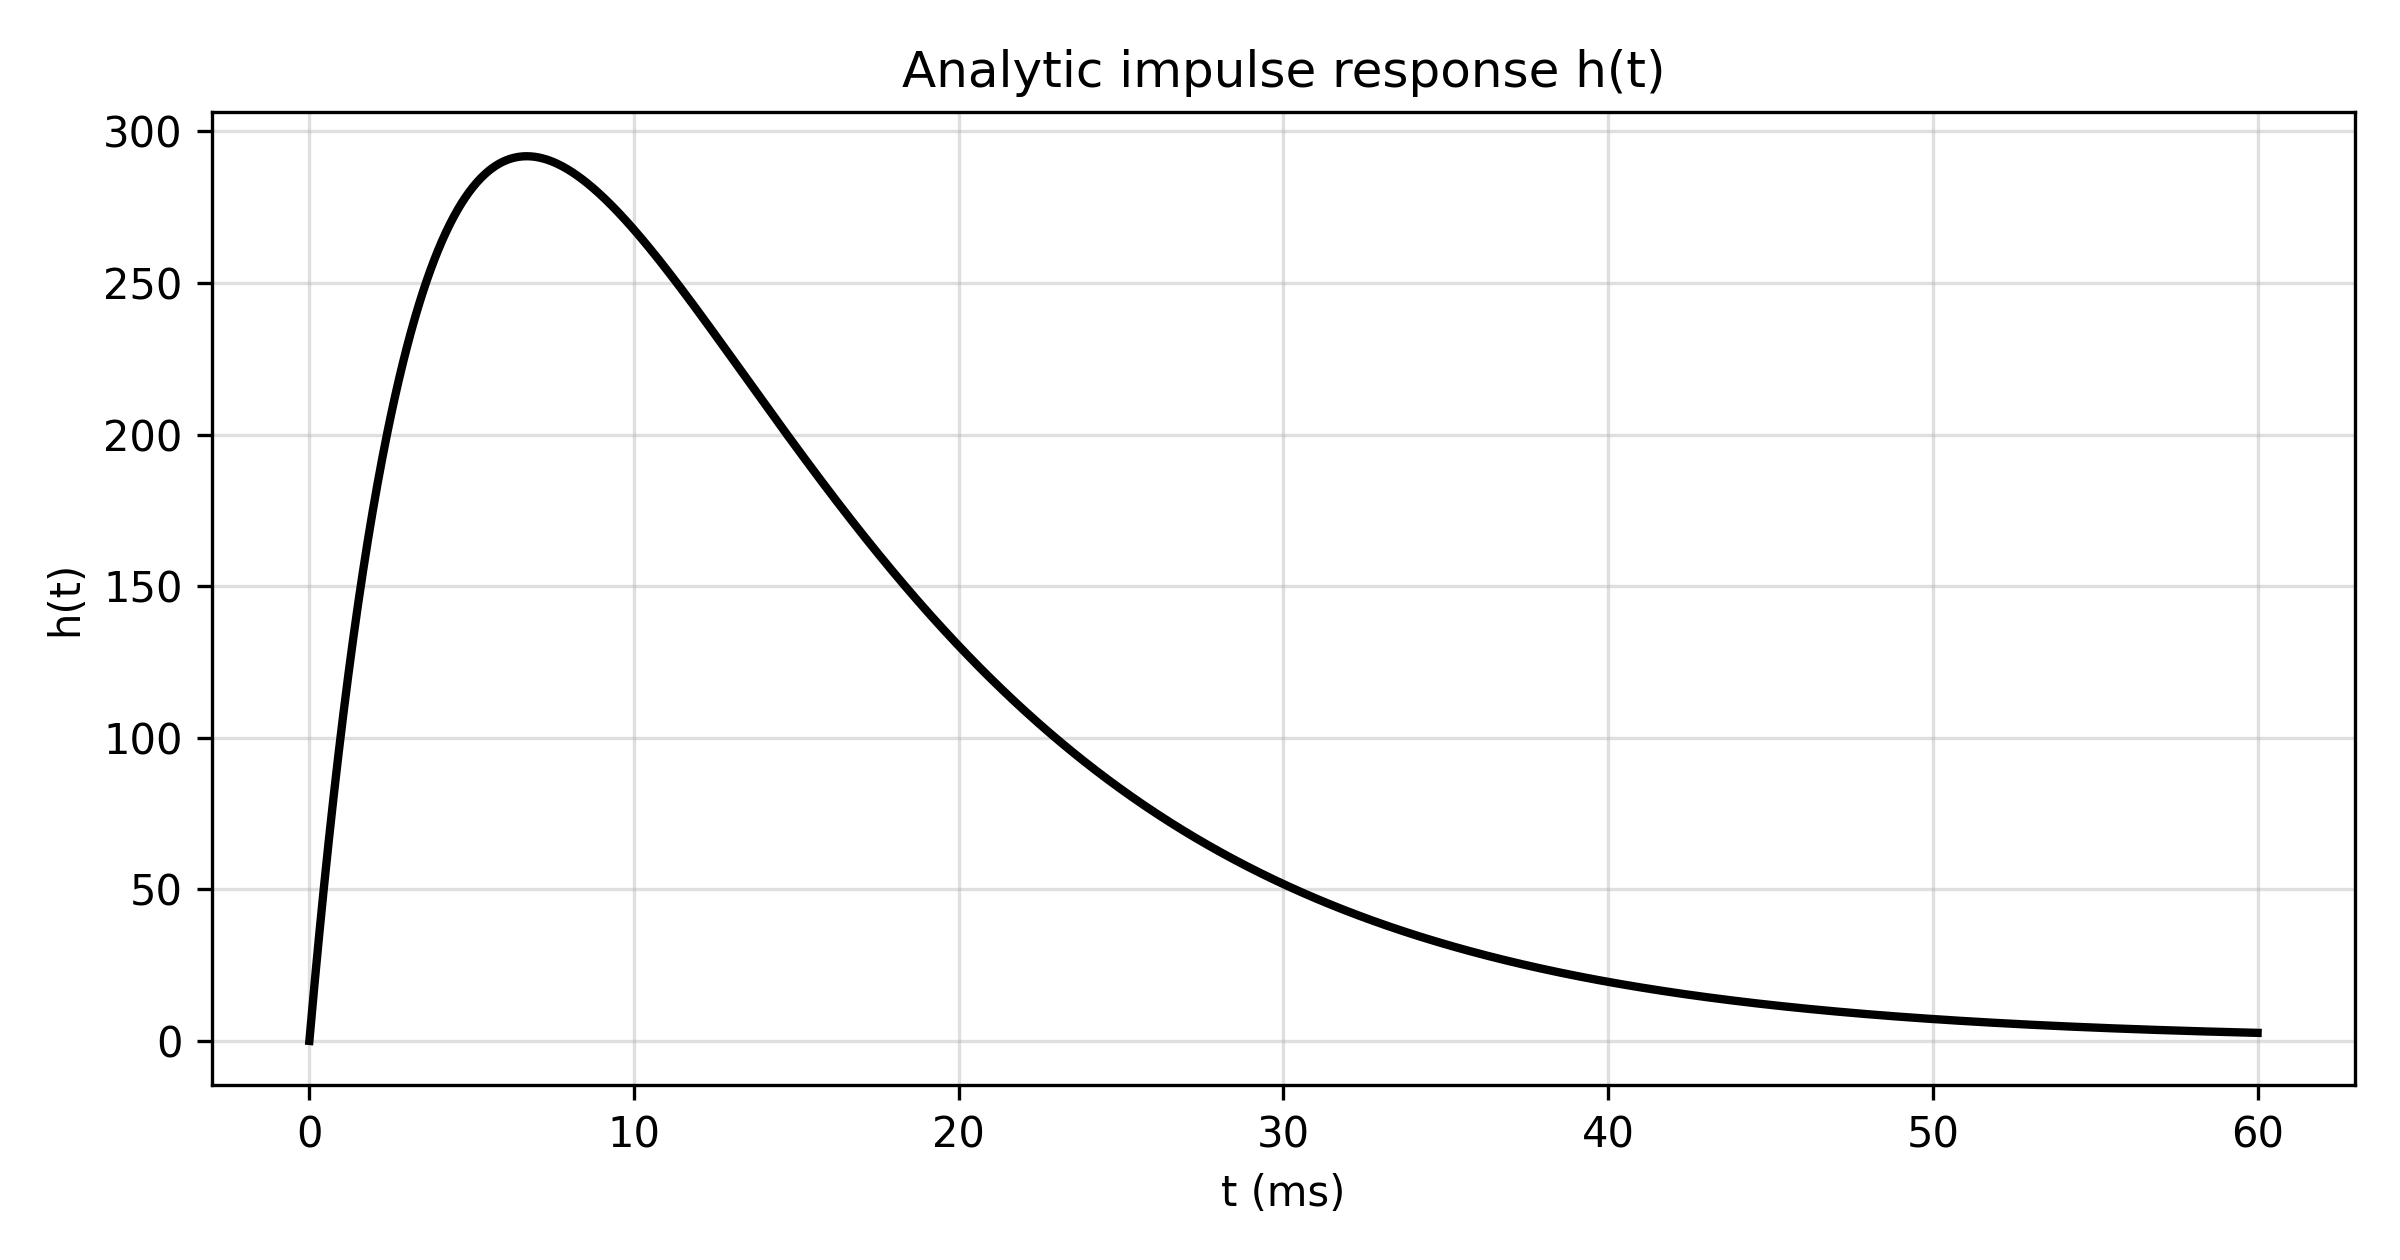
\includegraphics[width=0.8\textwidth]{h_analytic.png}
    \caption{Analytic impulse response $h(t)$.}
    \label{fig:h_analytic}
\end{figure}

\subsection*{4. Step response $s(t)$}
\addcontentsline{toc}{subsection}{Step response}
\begin{align*}
s(t) &= \int_0^t h(\sigma)\,d\sigma = \frac{G}{\tau_1 - \tau_2}\int_0^t \left(e^{-\sigma/\tau_1} - e^{-\sigma/\tau_2}\right)d\sigma \\
&= \frac{G}{\tau_1 - \tau_2}\Big[-\tau_1 e^{-\sigma/\tau_1} + \tau_2 e^{-\sigma/\tau_2}\Big]_{\sigma=0}^{\sigma=t} \\
&= \frac{G}{\tau_1 - \tau_2}\Big[-\tau_1 e^{-t/\tau_1} + \tau_2 e^{-t/\tau_2} + \tau_1 - \tau_2\Big]
\end{align*}
\[
\boxed{s(t) = \frac{G}{\tau_1 - \tau_2}\Big[\tau_1\left(1 - e^{-t/\tau_1}\right) + \tau_2\left(e^{-t/\tau_2} - 1\right)\Big]}
\]

\subsection*{5. DC gain}
\addcontentsline{toc}{subsection}{DC gain}
As $t \to \infty$ both exponentials go to zero:
\[
\lim_{t\to\infty}s(t) = \frac{G}{\tau_1 - \tau_2}\big[\tau_1 - \tau_2\big] = G = 1 + \frac{R_5}{R_4}.
\]

\subsection*{6. Pulse response by superposition}
\addcontentsline{toc}{subsection}{Superposition}
A rectangular pulse of height $A$ and width $T$ is the difference of two shifted steps:
\[
v_{in}(t) = A\,u(t) - A\,u(t-T) =
\begin{cases}
A, & 0 \le t < T \\
0, & \text{otherwise.}
\end{cases}
\]
The circuit is linear (its ODEs are linear) and time-invariant (the coefficients are constant), so scaling an input scales the output and delaying an input delays the output by the same amount. The response to a unit step is $s(t)$, so
\[
A\,u(t) - A\,u(t-T) \;\xrightarrow{\text{LTI system}}\; A\,s(t) - A\,s(t-T),
\]
and therefore
\[
\boxed{v_{out}(t) = A\big[s(t) - s(t-T)\big]}
\]

\subsection*{7. $v_{out}(t)$ using $s(t)$}
\addcontentsline{toc}{subsection}{Pulse response}
For $0 \le t < T$, $s(t-T) = 0$, so $v_{out}(t) = A\,s(t)$. For $t \ge T$:
\begin{align*}
v_{out}(t) &= A\big[s(t) - s(t-T)\big] \\
&= \frac{AG}{\tau_1 - \tau_2}\Big(\big[\tau_1(1 - e^{-t/\tau_1}) + \tau_2(e^{-t/\tau_2} - 1)\big] \\
&\qquad\qquad - \big[\tau_1(1 - e^{-(t-T)/\tau_1}) + \tau_2(e^{-(t-T)/\tau_2} - 1)\big]\Big) \\
&= \frac{AG}{\tau_1 - \tau_2}\Big[\tau_1\left(e^{-(t-T)/\tau_1} - e^{-t/\tau_1}\right) + \tau_2\left(e^{-t/\tau_2} - e^{-(t-T)/\tau_2}\right)\Big]
\end{align*}

\subsection*{8. Maximum $T$ for 1\% error}
\addcontentsline{toc}{subsection}{Maximum T}
From Section 1.2, a 1\% error requires $T \lesssim 0.02\,\tau$, where $\tau$ is the smallest time constant of the system. Here the smallest time constant is $\tau_2 = \SI{4.7e-3}{\second}$, so
\[
T \lesssim 0.02\,(\SI{4.7e-3}{\second}) = \SI{9.4e-5}{\second} = \SI{94}{\micro\second}.
\]

%---------------------------------------------------------------------
\newpage
\section*{Task 2.2: Rectangular Pulses}
\addcontentsline{toc}{section}{Task 2.2}

% Plots for T = 100 us, 1 ms, 10 ms, 50 ms (A = 1 V)
\begin{figure}[H]
    \centering
    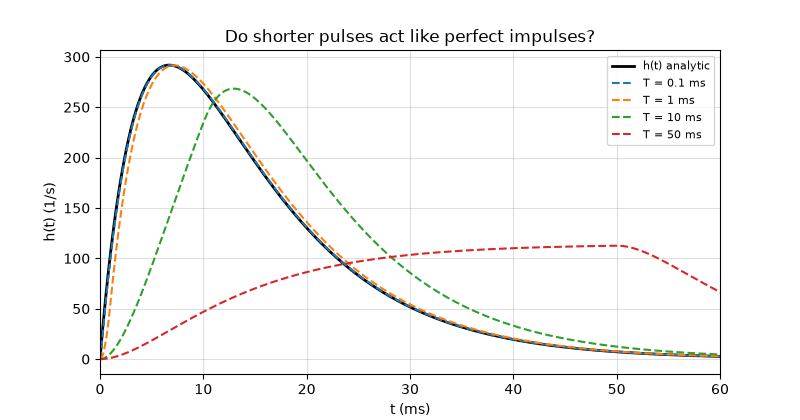
\includegraphics[width=0.9\textwidth]{task2.2_impulse.png}
    \caption{Four pulse widths compared to the analytic $h(t)$}
    \label{fig:rect_pulses}
\end{figure}


\subsection*{Which $T$ values collapse onto $h(t)$}
\addcontentsline{toc}{subsection}{Collapse onto h(t)}
Figure \ref{fig:rect_pulses} shows the output divided by the pulse area ($A\cdot T$) for four different pulse widths, plotted against the analytic $h(t)$. The shortest pulse, $T = 0.1$ ms collapsed almost perfectly onto $h(t)$, while the second shortest pulse, $T = 1$ ms, stays quite close to $h(t)$ and has the same overall shape, making it also work as a decent approximation of the impulse response. The 10 ms and 50 ms pulses do not collapse onto $h(t)$ at all. The 10 ms curve peaks lower and later than $h(t)$, and the 50 ms curve just slowly rises to a flat spot around 110 before falling off, which looks a lot more like a step response than an impulse response.

This lines up with the rule $T \lesssim 0.02\,\tau_{min}$. The smallest time constant is $\tau_2 = 4.7$ ms, so the pulse needs to be shorter than $0.02(4.7\text{ ms}) \approx 94\ \mu\text{s}$ to be within 1\% of $h(t)$. The 0.1 ms pulse is right at that limit, so it matches best. The 1 ms pulse is about 10 times over the limit, so it is close but a little off (roughly 5 to 10\% error). The 10 ms and 50 ms pulses are far over the limit, so they are nowhere near $h(t)$. Basically, the pulse has to be much shorter than the circuit's time constants. If it is not, the circuit has time to respond while the pulse is still on, and the output is no longer just the impulse response.

\subsection*{Effect of amplitude ($A = 5$ V vs.\ $A = 1$ V, $T = 100$ ms)}
\addcontentsline{toc}{subsection}{Amplitude comparison}
\begin{figure}[H]
    \centering
    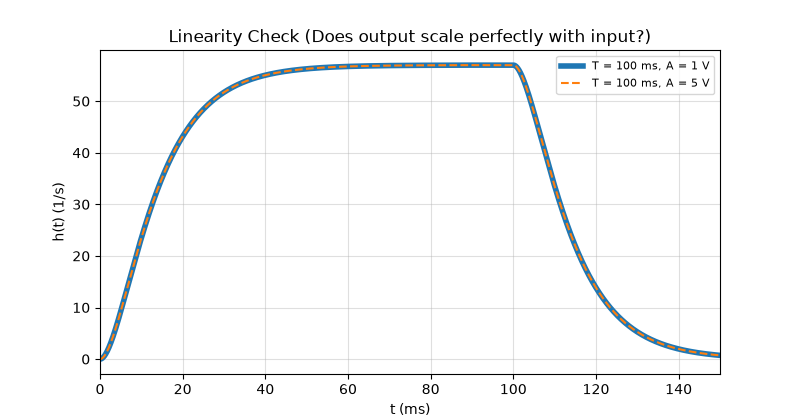
\includegraphics[width=0.9\textwidth]{task2.2_linear.png}
    \caption{Area-normalized response for $A=5$ V and $A=1$ V at $T=100$ ms.}
    \label{fig:amp_compare}
\end{figure}
In Figure \ref{fig:amp_compare}, the $A = 1$ V and $A = 5$ V curves land right on top of each other so the area-normalized curves are identical (the only difference is tiny numerical error from the solver). This shows that the system is linear. When the input gets 5 times bigger, the output also gets exactly 5 times bigger, so dividing by $A\cdot T$ cancels the amplitude out and same curve both times. The flat part of the curves sits at about 57, which is $G/T = 5.7/0.1$ s. This makes sense because the output settles at the DC gain $G$ times the input before the pulse ends. Neither curve matches $h(t)$ because 100 ms is way too long to act like an impulse, but that is fine since this test is only checking linearity.

%---------------------------------------------------------------------
\newpage
\newpage
\section*{Task 2.3: Triangular Pulse}
\addcontentsline{toc}{section}{Task 2.3}

For this task, the rectangular input was swapped for a triangular pulse with $T = 100\ \mu$s and a peak of $A = 2$ V. The parts of the code that changed are below: the input array for plotting, the input inside \texttt{f\_rhs} so the solver sees the triangle, and the normalization by the triangle's area.

\begin{lstlisting}[style=python, caption={Modified code for triangular input}]
A = 2.0          # peak of triangle (V)
T = 100e-6       # pulse width (s)

# triangular input array (for plotting)
vin = np.zeros(len(t_eval))
for i, t in enumerate(t_eval):
    if 0 <= t <= T/2:
        vin[i] = (2 * A / T) * t
    elif T/2 < t <= T:
        vin[i] = (2 * A / T) * (T - t)

# triangular input inside f_rhs so the solver sees it
def f_rhs(t, x):
    v1, v2 = x
    if 0 <= t <= T/2:
        _vin = (2 * A / T) * t
    elif T/2 < t <= T:
        _vin = (2 * A / T) * (T - t)
    else:
        _vin = 0.0
    return [(_vin - v1)/tau1, (G*v1 - v2)/tau2]

# normalize by triangle area = 0.5*A*T
area = 0.5 * A * T
axn.plot(t_eval * 1e3, v2 / area, "--", color="orange", label="Normalized Triangle")
\end{lstlisting}

\begin{figure}[H]
    \centering
    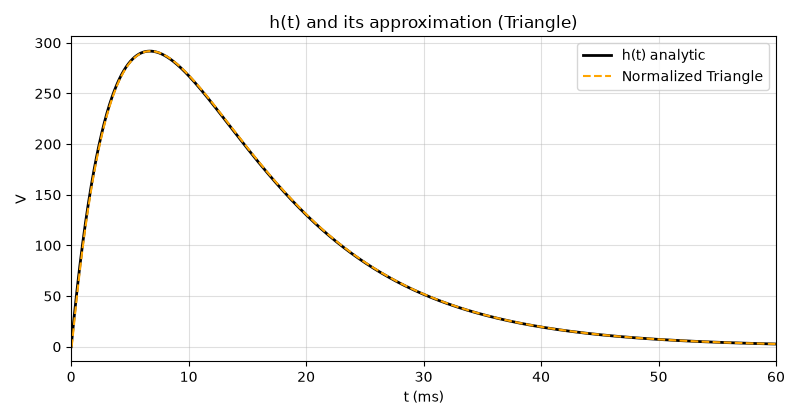
\includegraphics[width=0.9\textwidth]{2.3.png}
    \caption{Triangular input and $v_{c2}/(0.5AT)$ overlaid with $h(t)$.}
    \label{fig:tri_pulse}
\end{figure}

The triangle has an area of $\frac{1}{2}AT = \frac{1}{2}(2\text{ V})(100\ \mu\text{s}) = 1\times10^{-4}$ V$\cdot$s, which is the same as the 1 V, 100 $\mu$s rectangle from Task 2.2. Figure \ref{fig:tri_pulse} shows the output divided by that area, and it lands right on top of $h(t)$. The peak is about 292 at around 6.7 ms, same as $h(t)$, and it stays within about 0.5\% of $h(t)$ for the rest of the curve. So no, the shape of the pulse does not matter as long as the area is the same (and the pulse is short enough).

The math behind this is that the output is the input convolved with $h(t)$:
\[
v_{c2}(t) = \int_0^T h(t-\tau)\,v_{in}(\tau)\,d\tau.
\]
If $T$ is really short compared to the time constants, then $h(t-\tau)$ barely changes while the pulse is on, so $h(t-\tau) \approx h(t)$ for $0 \le \tau \le T$. That lets $h(t)$ be pulled out of the integral:
\[
v_{c2}(t) \approx h(t)\int_0^T v_{in}(\tau)\,d\tau = h(t)\cdot(\text{area of the pulse}).
\]
So the only thing about the input that shows up in the output is its area, not its shape. That is why dividing by the area gives $h(t)$ for both the rectangle ($AT$) and the triangle ($\frac{1}{2}AT$). The tiny difference that is left comes from the pulse not being infinitely short.

%---------------------------------------------------------------------
\newpage
\section*{Task 2.4: Step Response}
\addcontentsline{toc}{section}{Task 2.4}

For this task, the pulse was replaced with a step input of height $A = 1$ V that stays on for all $t \ge 0$. The modified parts of the code are below: the step input, the step inside \texttt{f\_rhs} so the solver sees it, and the derivative of the step response using \texttt{np.gradient()}.

\begin{lstlisting}[style=python, caption={Modified code for step input and differentiation}]
A = 1.0
t_end = 8 * tau_max          # no pulse now, so no T added
t_eval = np.linspace(0.0, t_end, 4000)
max_step = tau_min / 20.0

# step input is A for all t >= 0
vin = np.ones(len(t_eval)) * A

# f_rhs with a constant step input
def f_rhs(t, x):
    v1, v2 = x
    _vin = A                 # input is always A
    return [(_vin - v1)/tau1, (G*v1 - v2)/tau2]

sol = solve_ivp(f_rhs, (0.0, t_end), [0.0, 0.0], t_eval=t_eval, rtol=1e-8, atol=1e-8, max_step=max_step)
v2_step = sol.y[1]

# differentiate the step response
ds_dt = np.gradient(v2_step, t_eval)
\end{lstlisting}

\begin{figure}[H]
    \centering
    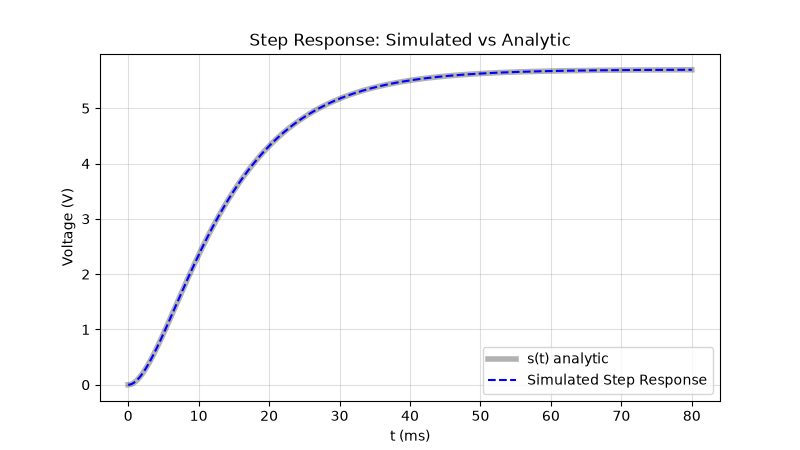
\includegraphics[width=0.9\textwidth]{2.4_step.png}
    \caption{Simulated step response with analytic $s(t)$ overlaid.}
    \label{fig:step_sim}
\end{figure}

\begin{figure}[H]
    \centering
    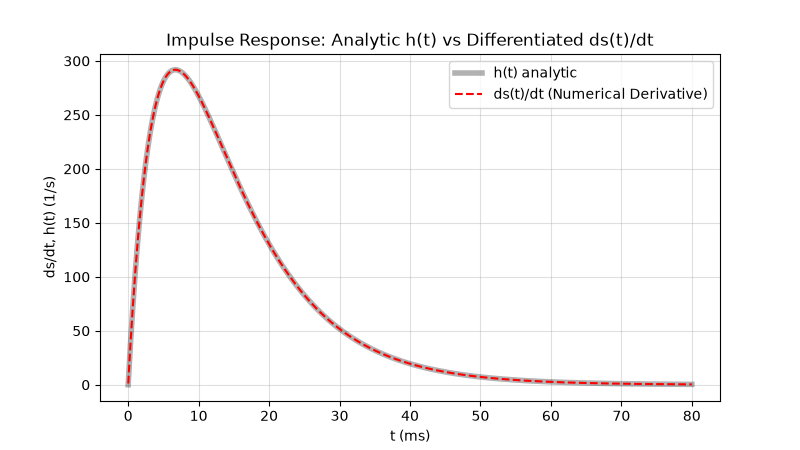
\includegraphics[width=0.9\textwidth]{2.4_impulse.png}
    \caption{$h(t)$ overlaid with $ds(t)/dt$ computed numerically.}
    \label{fig:step_deriv}
\end{figure}

Figure \ref{fig:step_sim} shows the simulated step response with the analytic $s(t)$ from Task 1 behind it. The two curves sit right on top of each other, so the simulation matches the math.

\subsection*{Are $h(t)$ and $ds(t)/dt$ the same?}
\addcontentsline{toc}{subsection}{h(t) vs ds/dt}
Yes. In Figure \ref{fig:step_deriv}, the numerical derivative of the step response lands right on top of the analytic $h(t)$. This makes sense because the step response is the integral of the impulse response,
\[
s(t) = \int_0^t h(\sigma)\,d\sigma,
\]
so taking the derivative of $s(t)$ just gives $h(t)$ back:
\[
\frac{ds(t)}{dt} = h(t).
\]


\subsection*{Final value and settling time}
\addcontentsline{toc}{subsection}{Final value and settling time}
The step response levels off at about 5.696 V by $t = 80$ ms, which is $G = 5.7$ to within 0.1\%. The tiny gap is just the last bit of the slow exponential not being gone yet. This matches the DC gain from Task 1, $G = 1 + R_5/R_4 = 5.7$, so a 1 V step ends up as 5.7 V at the output.

The settling time is mostly controlled by the slower time constant, $\tau_1 = 10$ ms. Writing $s(t)$ as
\[
s(t) = G - \frac{G}{\tau_1 - \tau_2}\left(\tau_1 e^{-t/\tau_1} - \tau_2 e^{-t/\tau_2}\right),
\]
the $e^{-t/\tau_2}$ term dies off faster, so at later times the gap to $G$ is mostly just the $e^{-t/\tau_1}$ term. From the simulation, the output gets within 2\% of $G$ at about 45 ms and within 1\% at about 52 ms. For a single RC circuit, 2\% settling would be about $4\tau_1 = 40$ ms, so the second stage makes it take a little longer. The faster time constant $\tau_2$ does not really set the settling time. It mostly shows up at the start, where the response begins flat and then curves upward instead of jumping up like a single RC circuit.

%---------------------------------------------------------------------
\newpage
\section*{Task 3.1: Build and Instrument}
\addcontentsline{toc}{section}{Task 3.1}
The RC opamp circuit was built before any measurements were taken and everything was looked over by the group, the first build of the circuit was not working properly, due to a swapped resistor making the gain not boost to 5.7. Once that was resolved the opamp was also replaced just to be safe and the output was amplified as expected.

\begin{figure}[H]
    \centering
     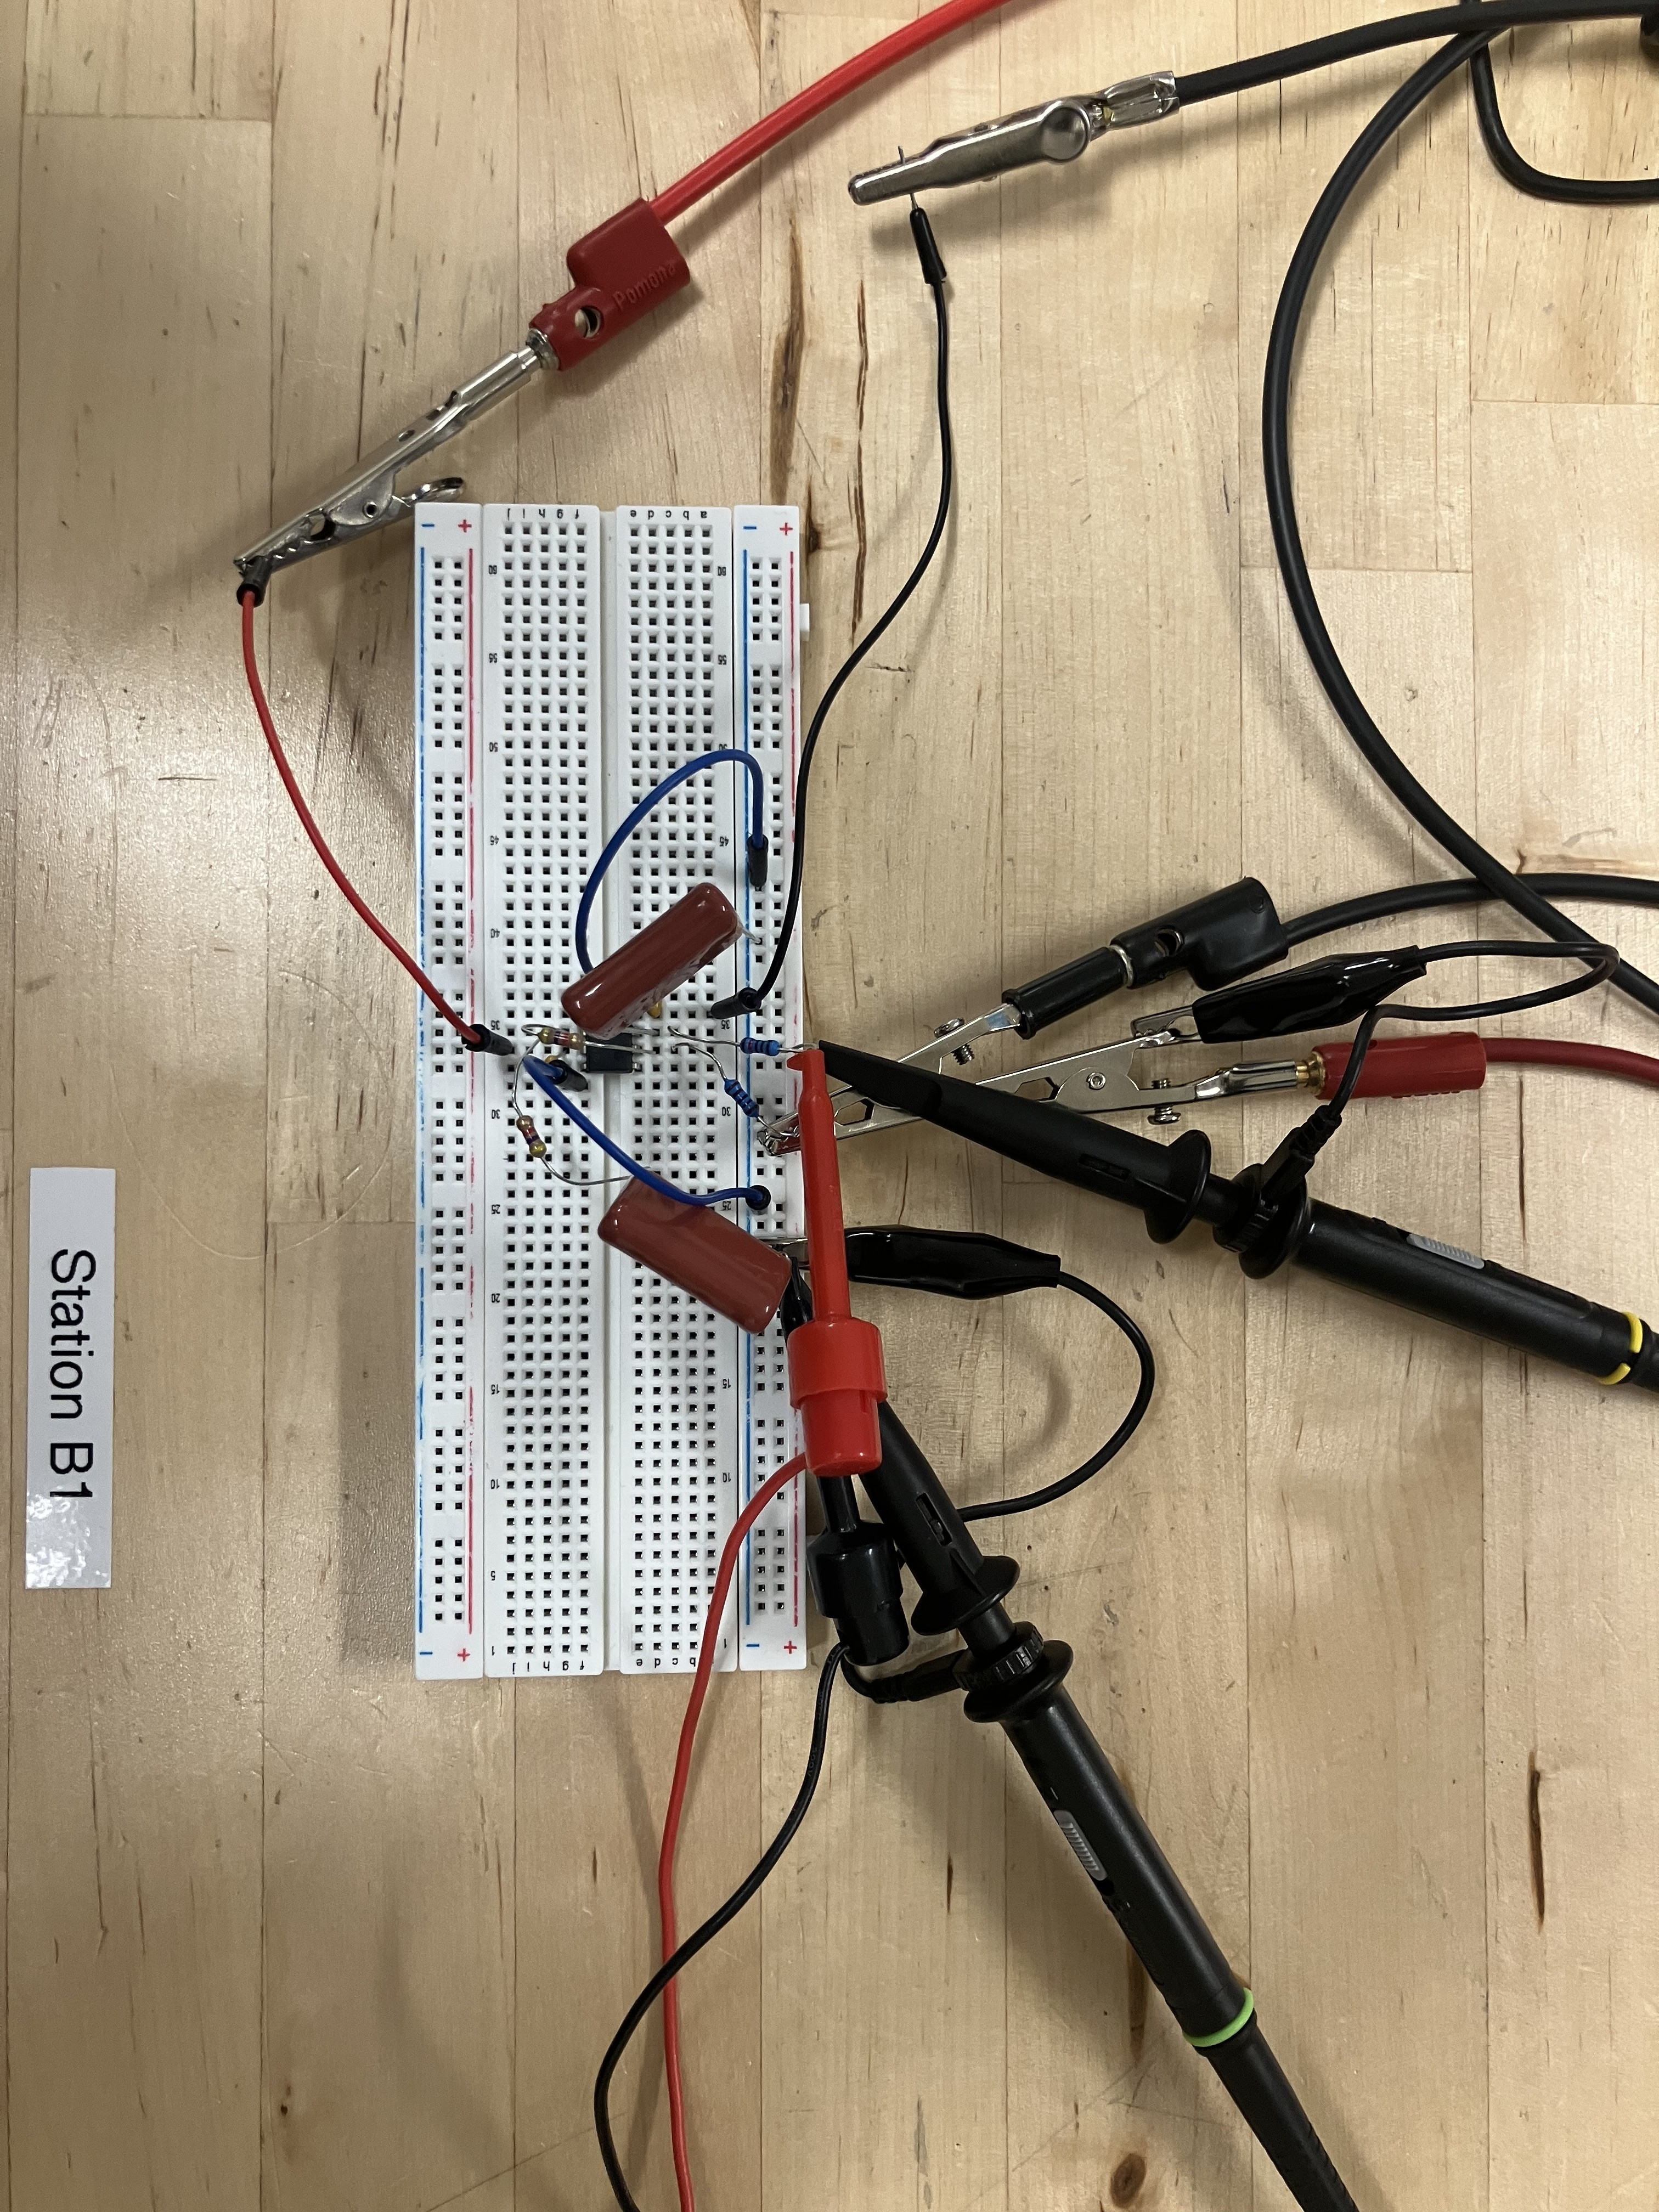
\includegraphics[width=0.6\textwidth]{circuit_construction.jpeg}
    \caption{RC Opamp Circuit on Breadboard.}
    \label{fig:breadboard}
\end{figure}

%---------------------------------------------------------------------
\newpage
\section*{Task 3.2: Impulse Response Measurements}
\addcontentsline{toc}{section}{Task 3.2}

% One slow + one fast capture for each setting:
\subsection*{5 V, 100 $\mu$s, 10 Hz}
\addcontentsline{toc}{subsection}{5 V, 100 us}
\begin{figure}[H]
    \centering
     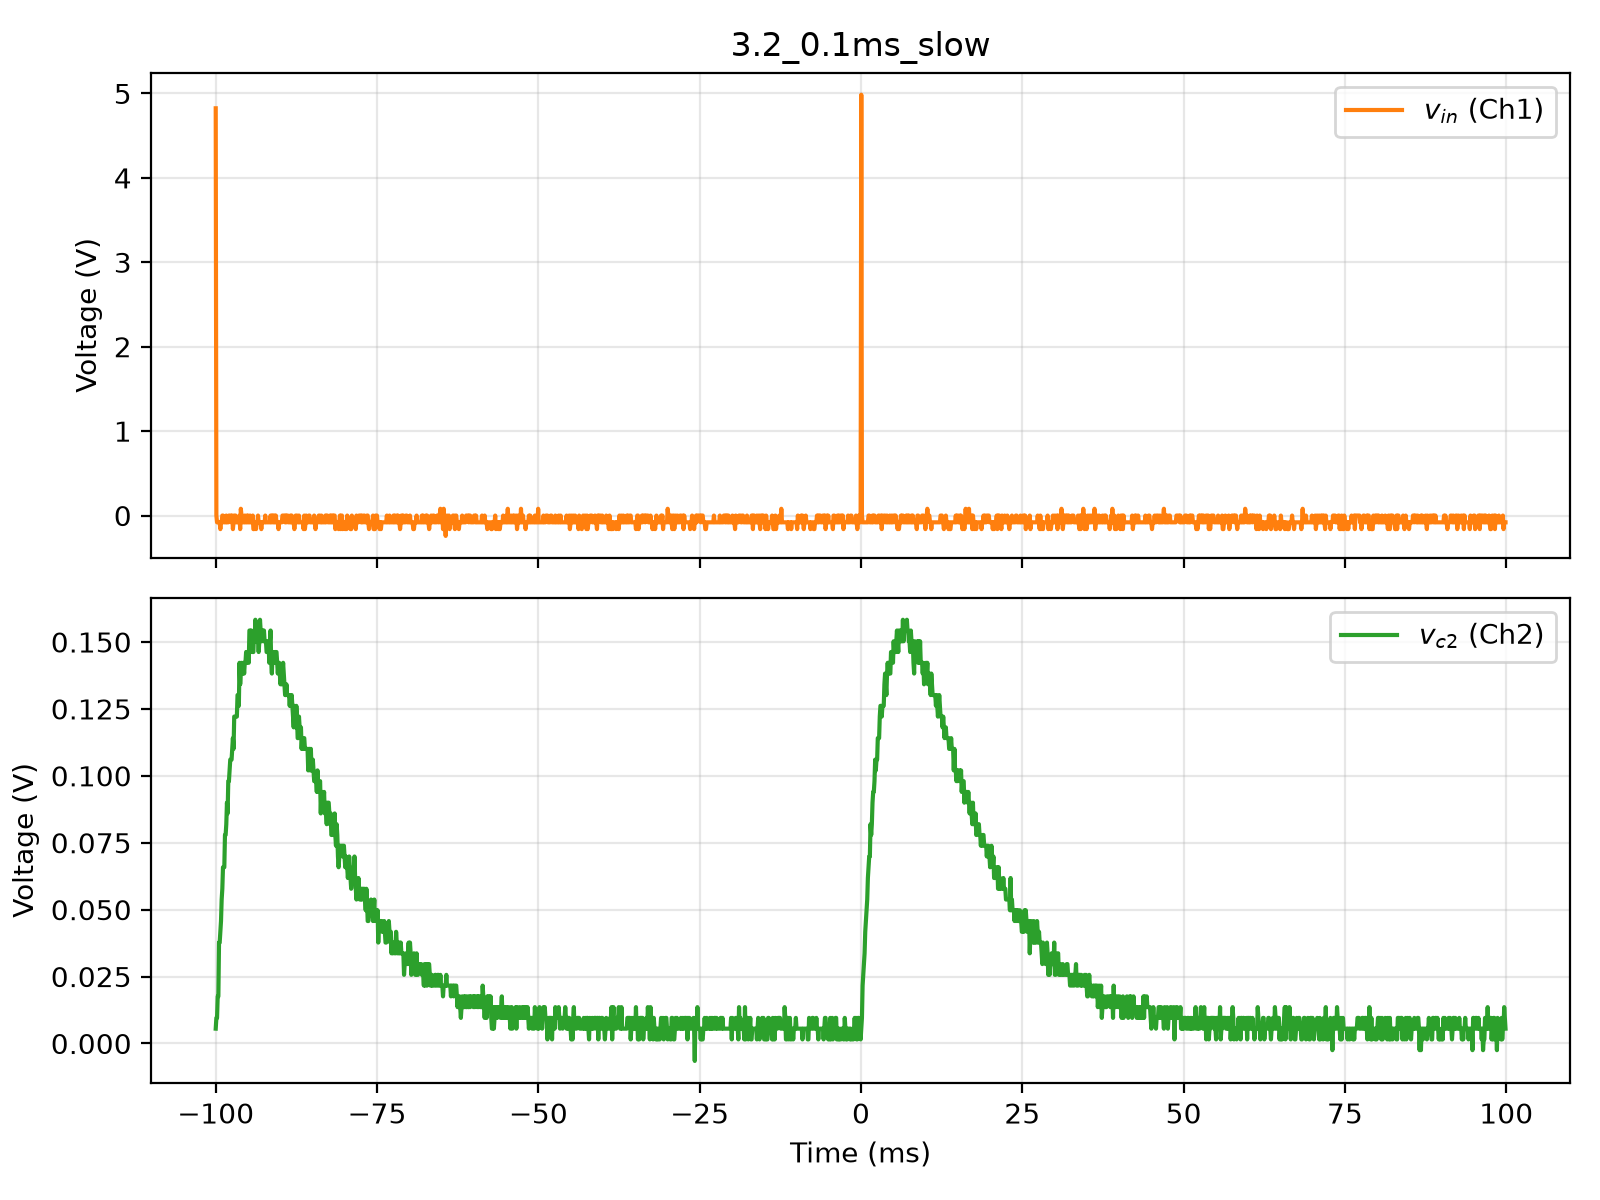
\includegraphics[width=0.48\textwidth]{3.2_0.1ms_slow.png}
    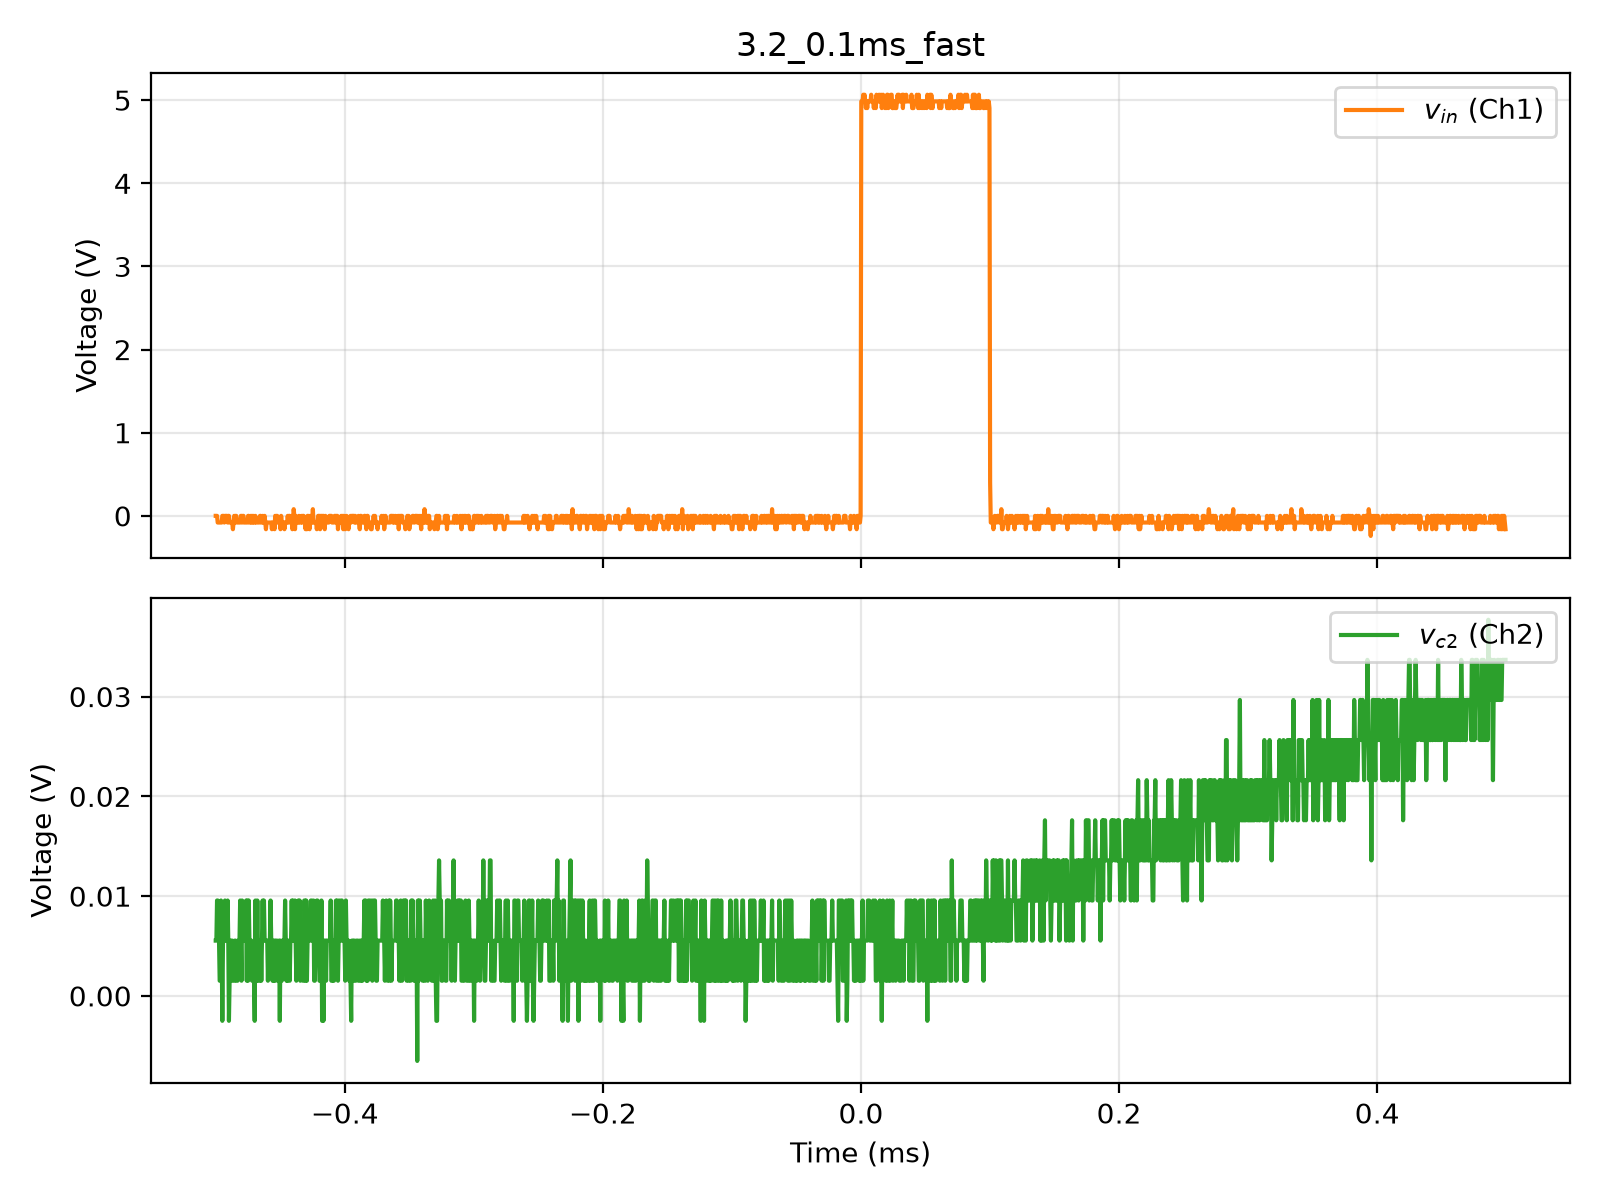
\includegraphics[width=0.48\textwidth]{3.2_0.1ms_fast.png}
    \caption{Slow and fast sweeps for the 100 $\mu$s pulse.}
    \label{fig:p100us}
\end{figure}

\subsection*{5 V, 1 ms, 10 Hz}
\addcontentsline{toc}{subsection}{5 V, 1 ms}
\begin{figure}[H]
    \centering
    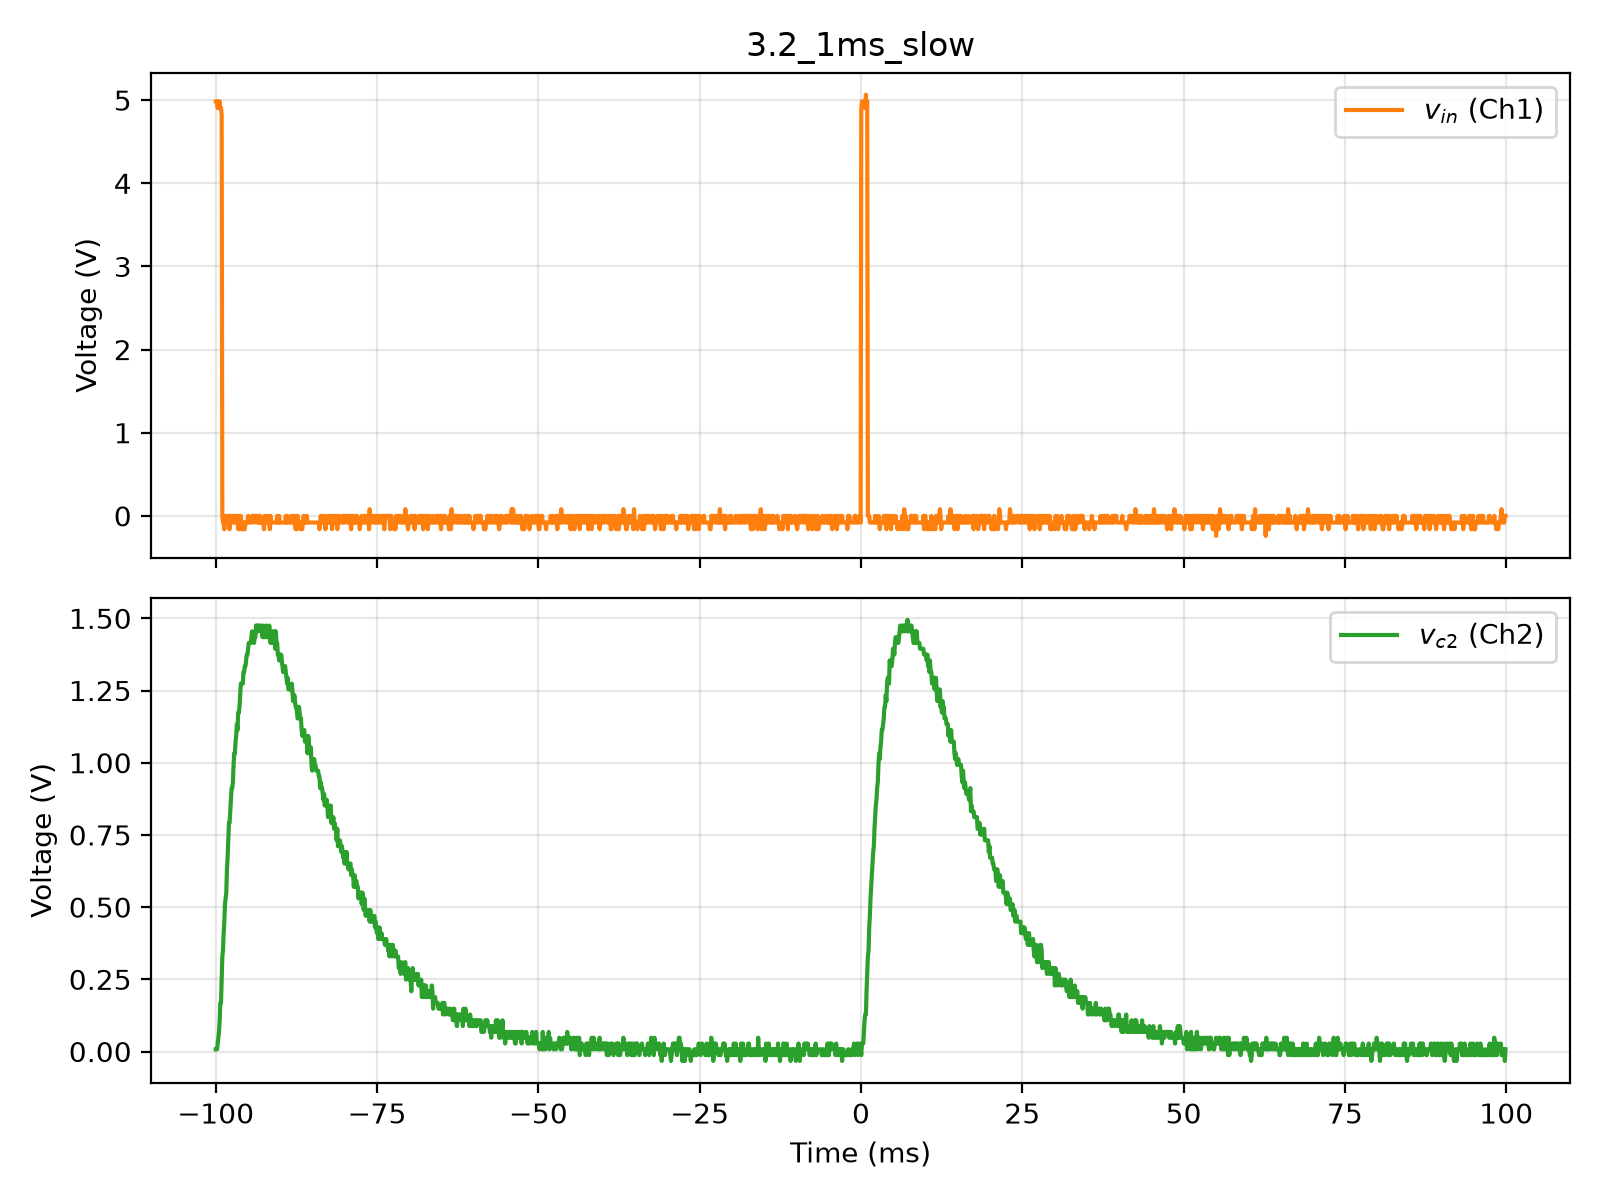
\includegraphics[width=0.48\textwidth]{3.2_1ms_slow.png}
    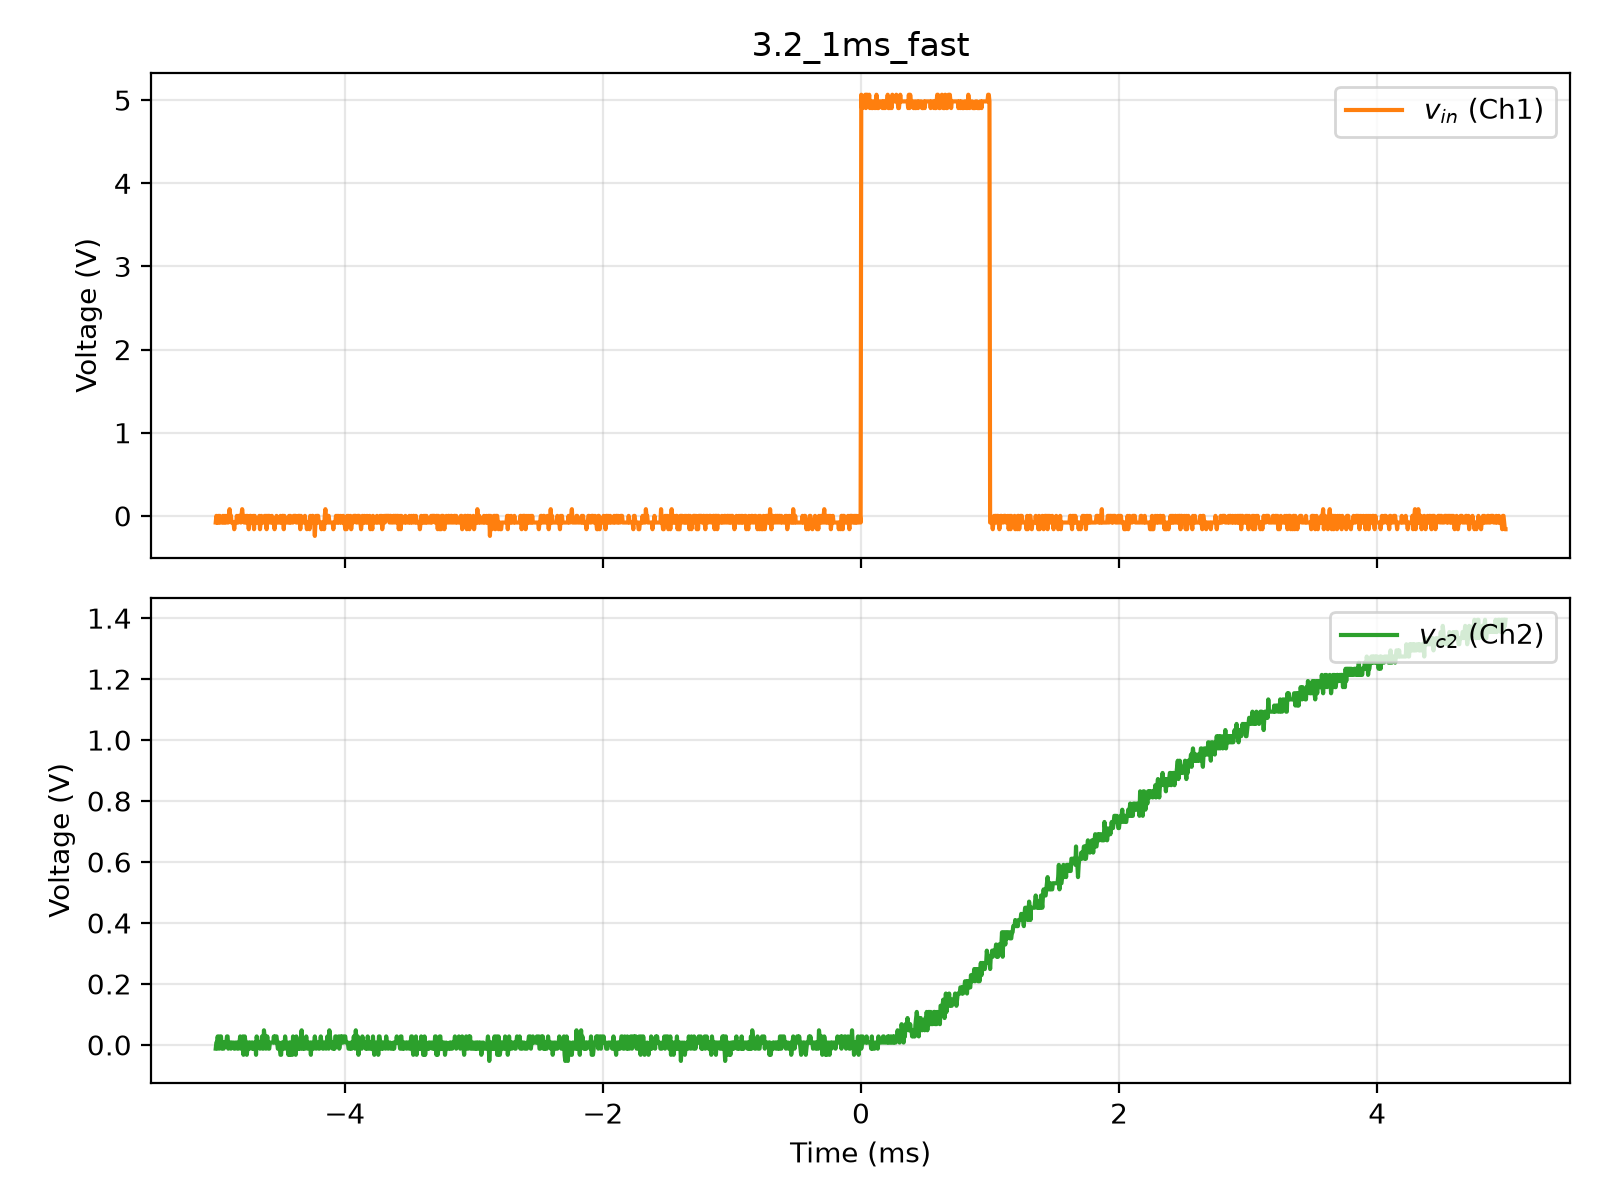
\includegraphics[width=0.48\textwidth]{3.2_1ms_fast.png}
    \caption{Slow and fast sweeps for the 1 ms pulse.}
    \label{fig:p1ms}
\end{figure}

\subsection*{2 V, 10 ms, 10 Hz}
\addcontentsline{toc}{subsection}{2 V, 10 ms}
\begin{figure}[H]
    \centering
     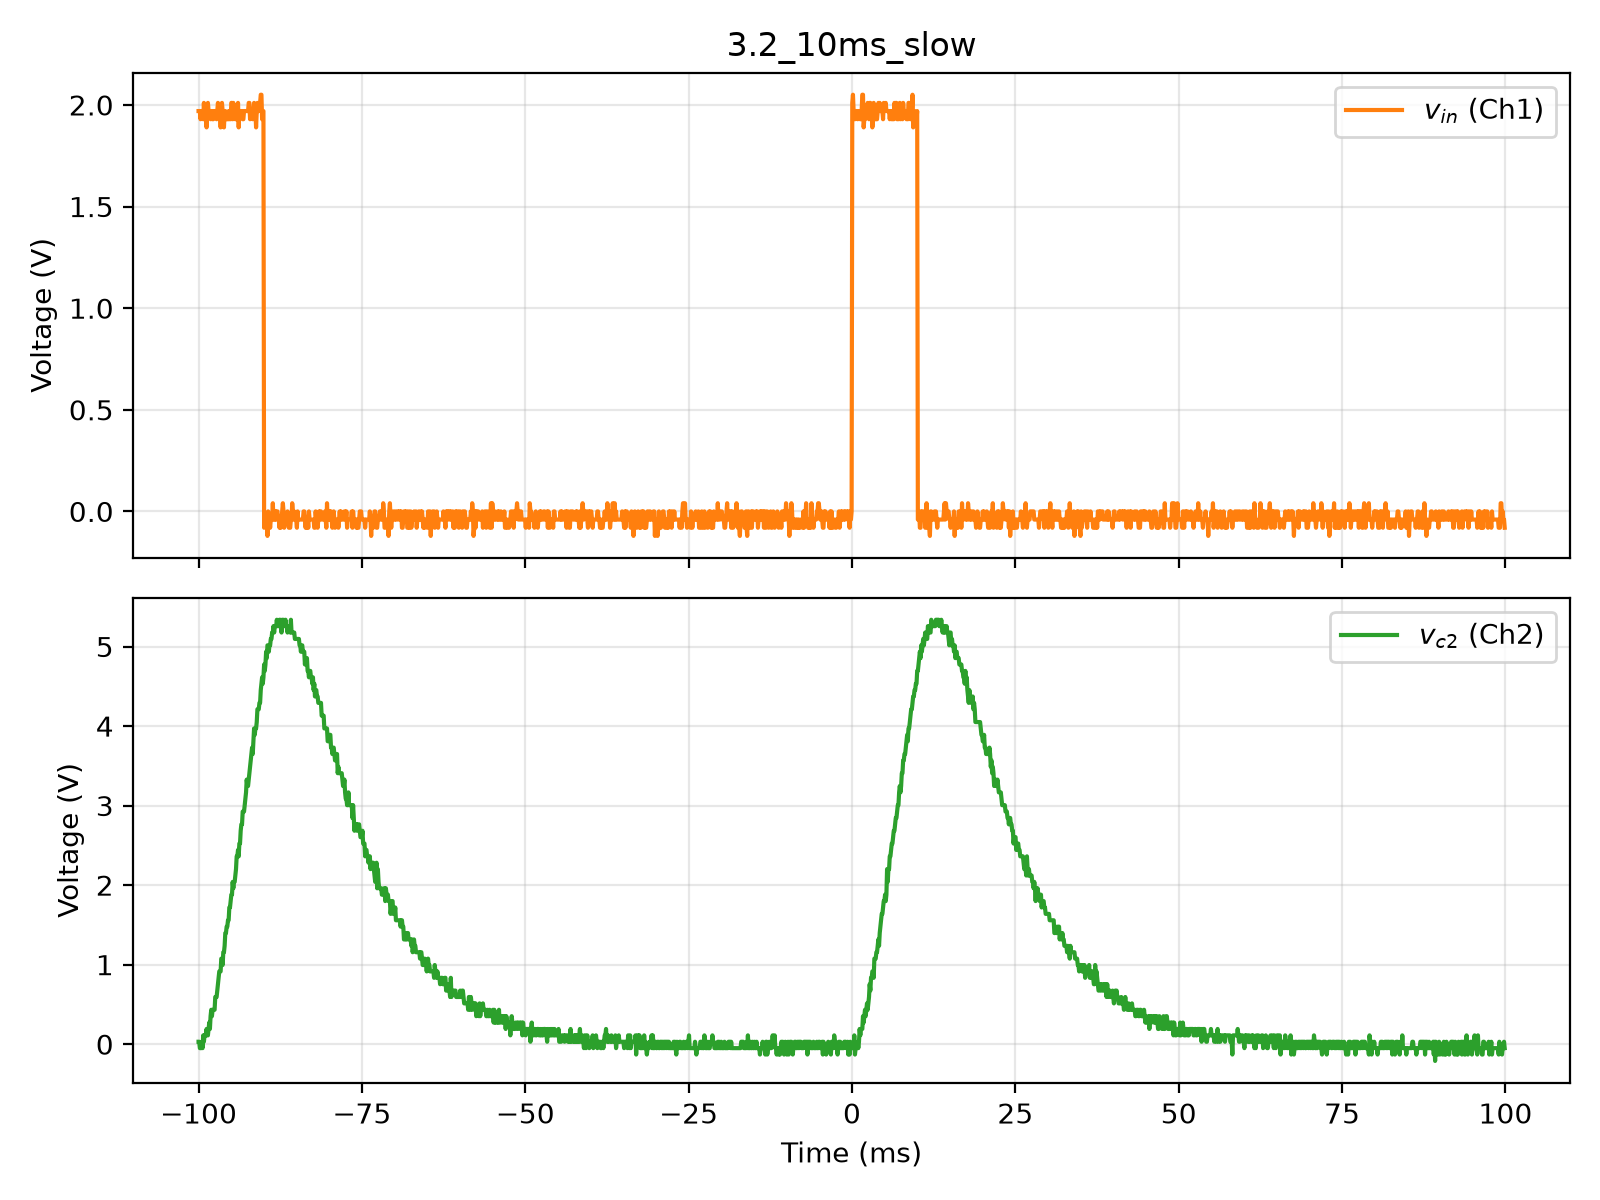
\includegraphics[width=0.48\textwidth]{3.2_10ms_slow.png}
    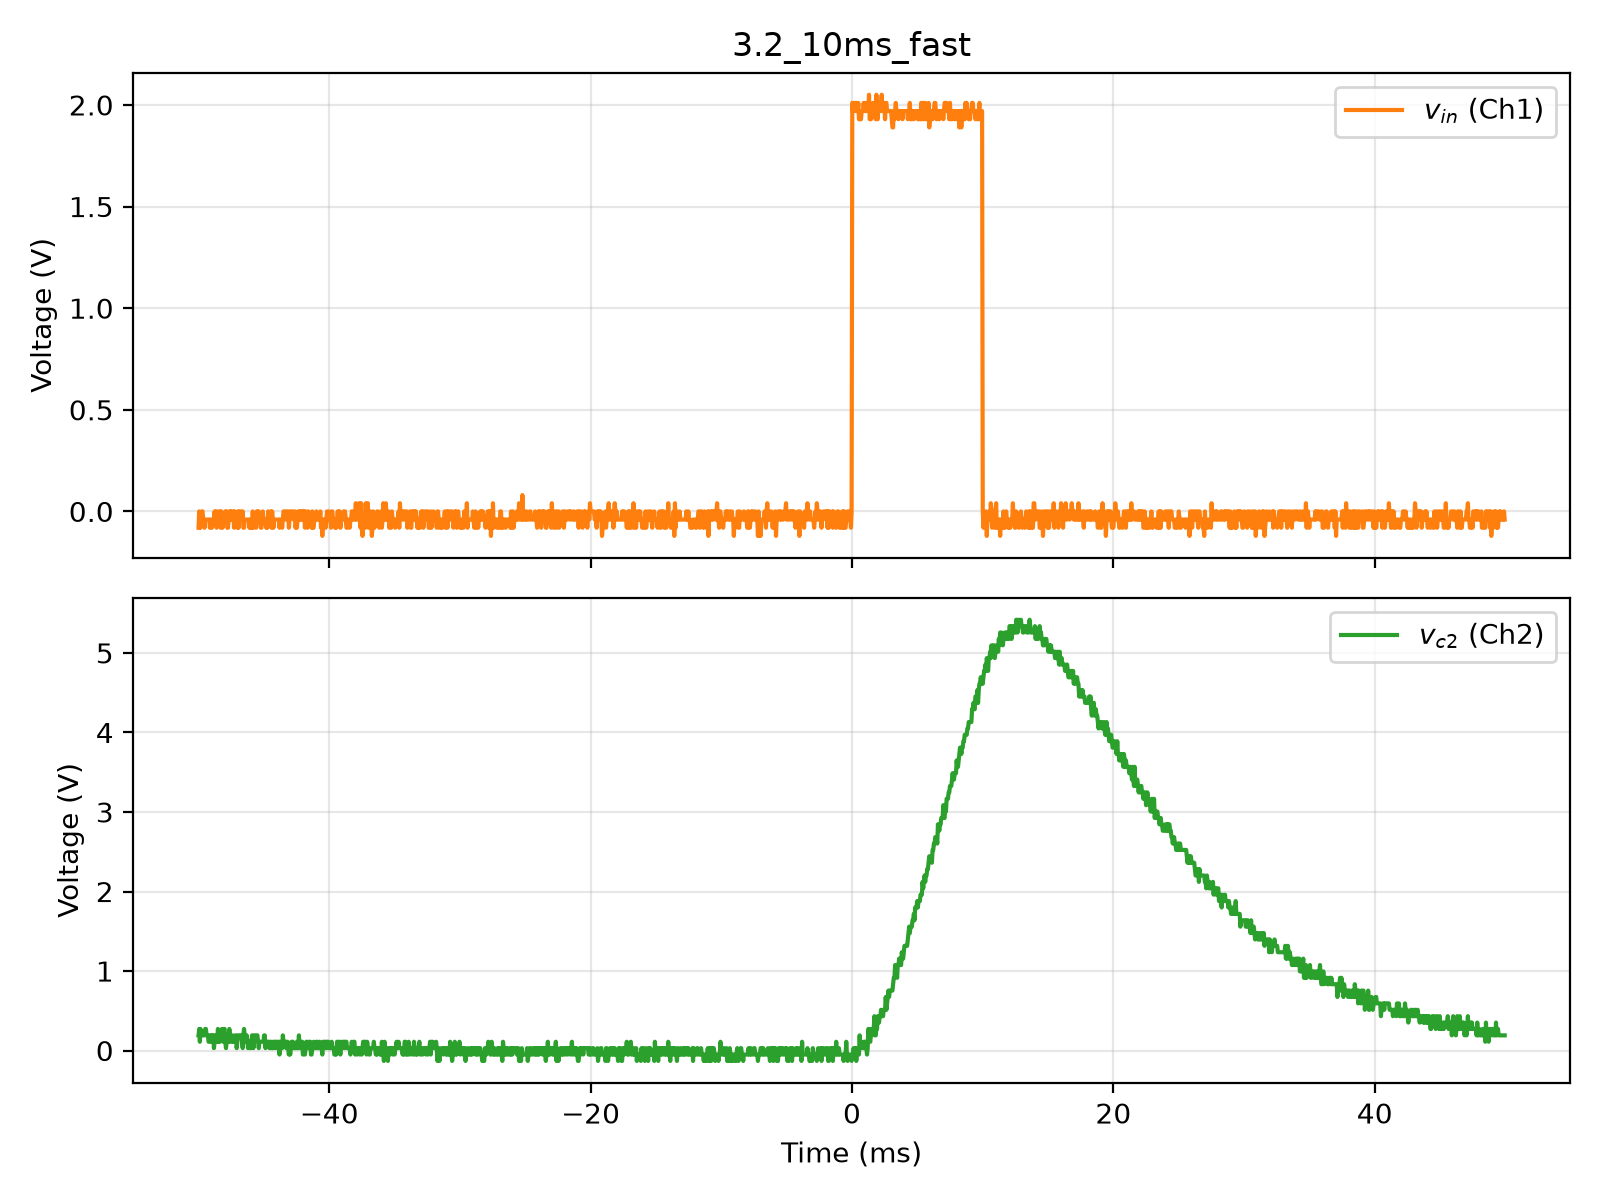
\includegraphics[width=0.48\textwidth]{3.2_10ms_fast.png}
    \caption{Slow and fast sweeps for the 10 ms pulse.}
    \label{fig:p10ms}
\end{figure}

\subsection*{2 V, 50 ms, 1 Hz}
\addcontentsline{toc}{subsection}{2 V, 50 ms}
\begin{figure}[H]
    \centering
     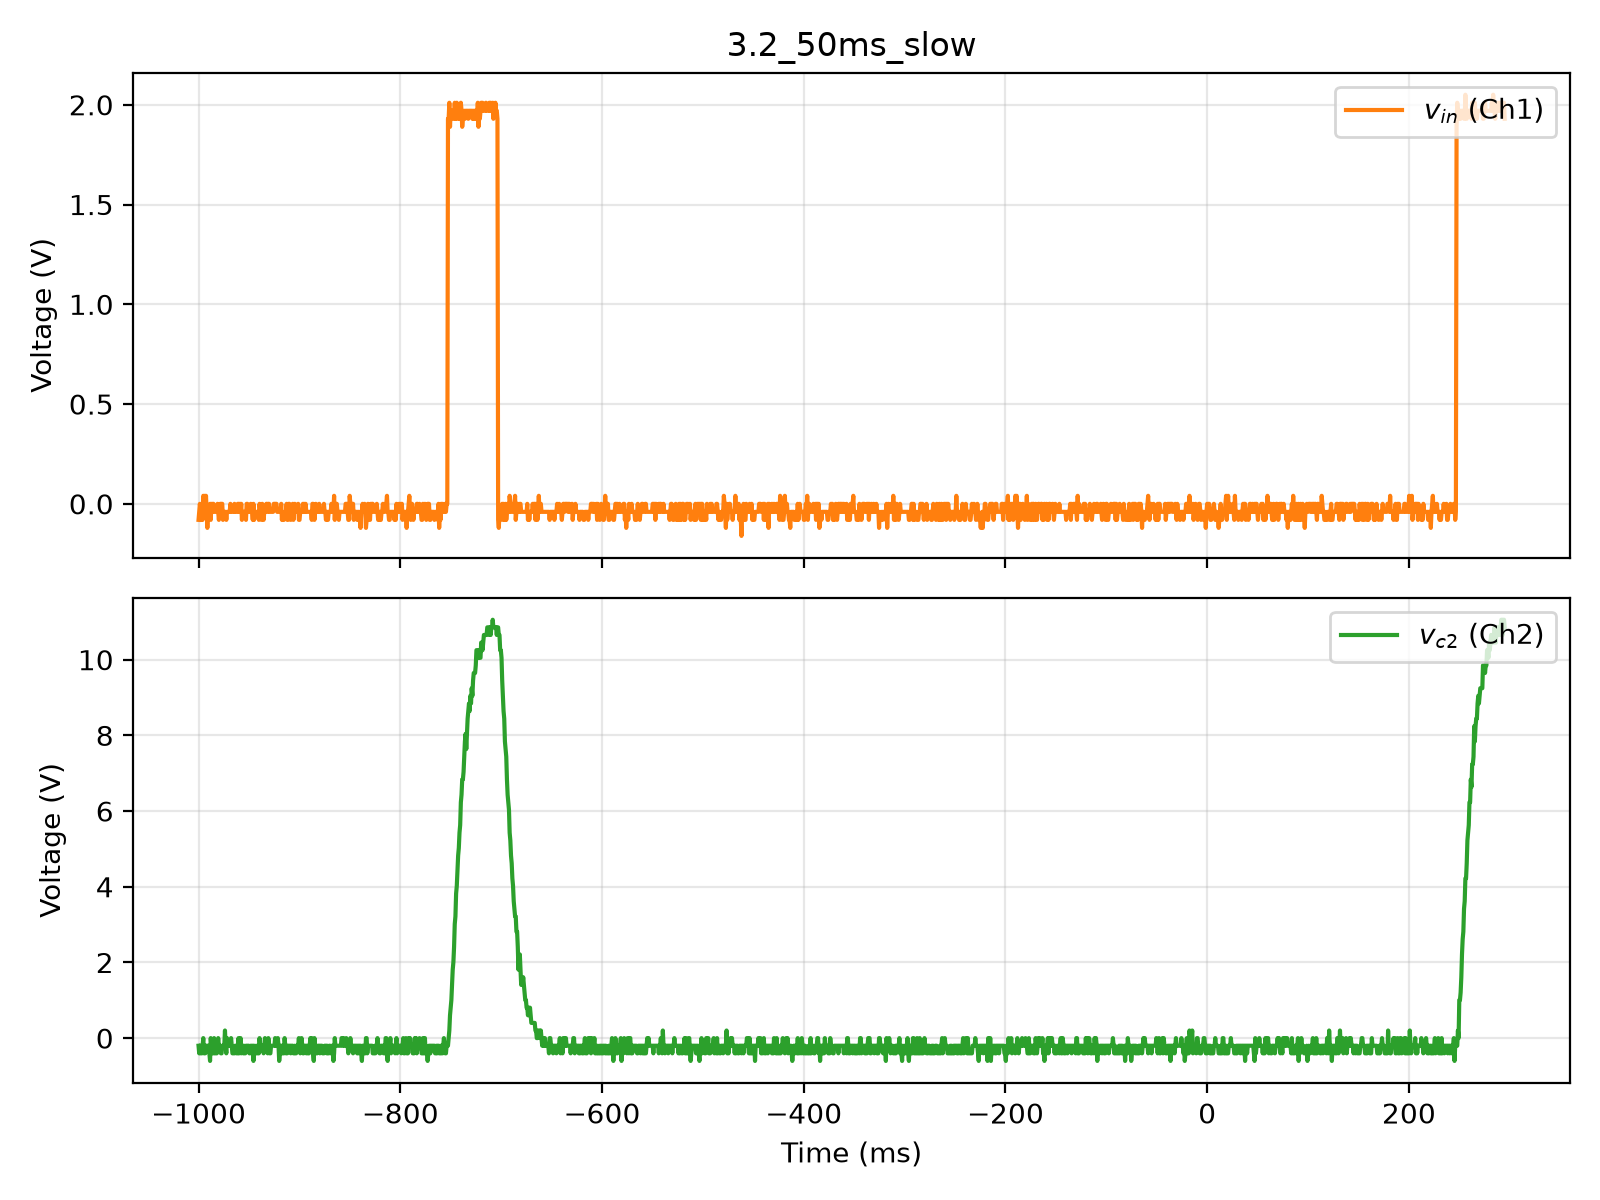
\includegraphics[width=0.48\textwidth]{3.2_50ms_slow.png}
     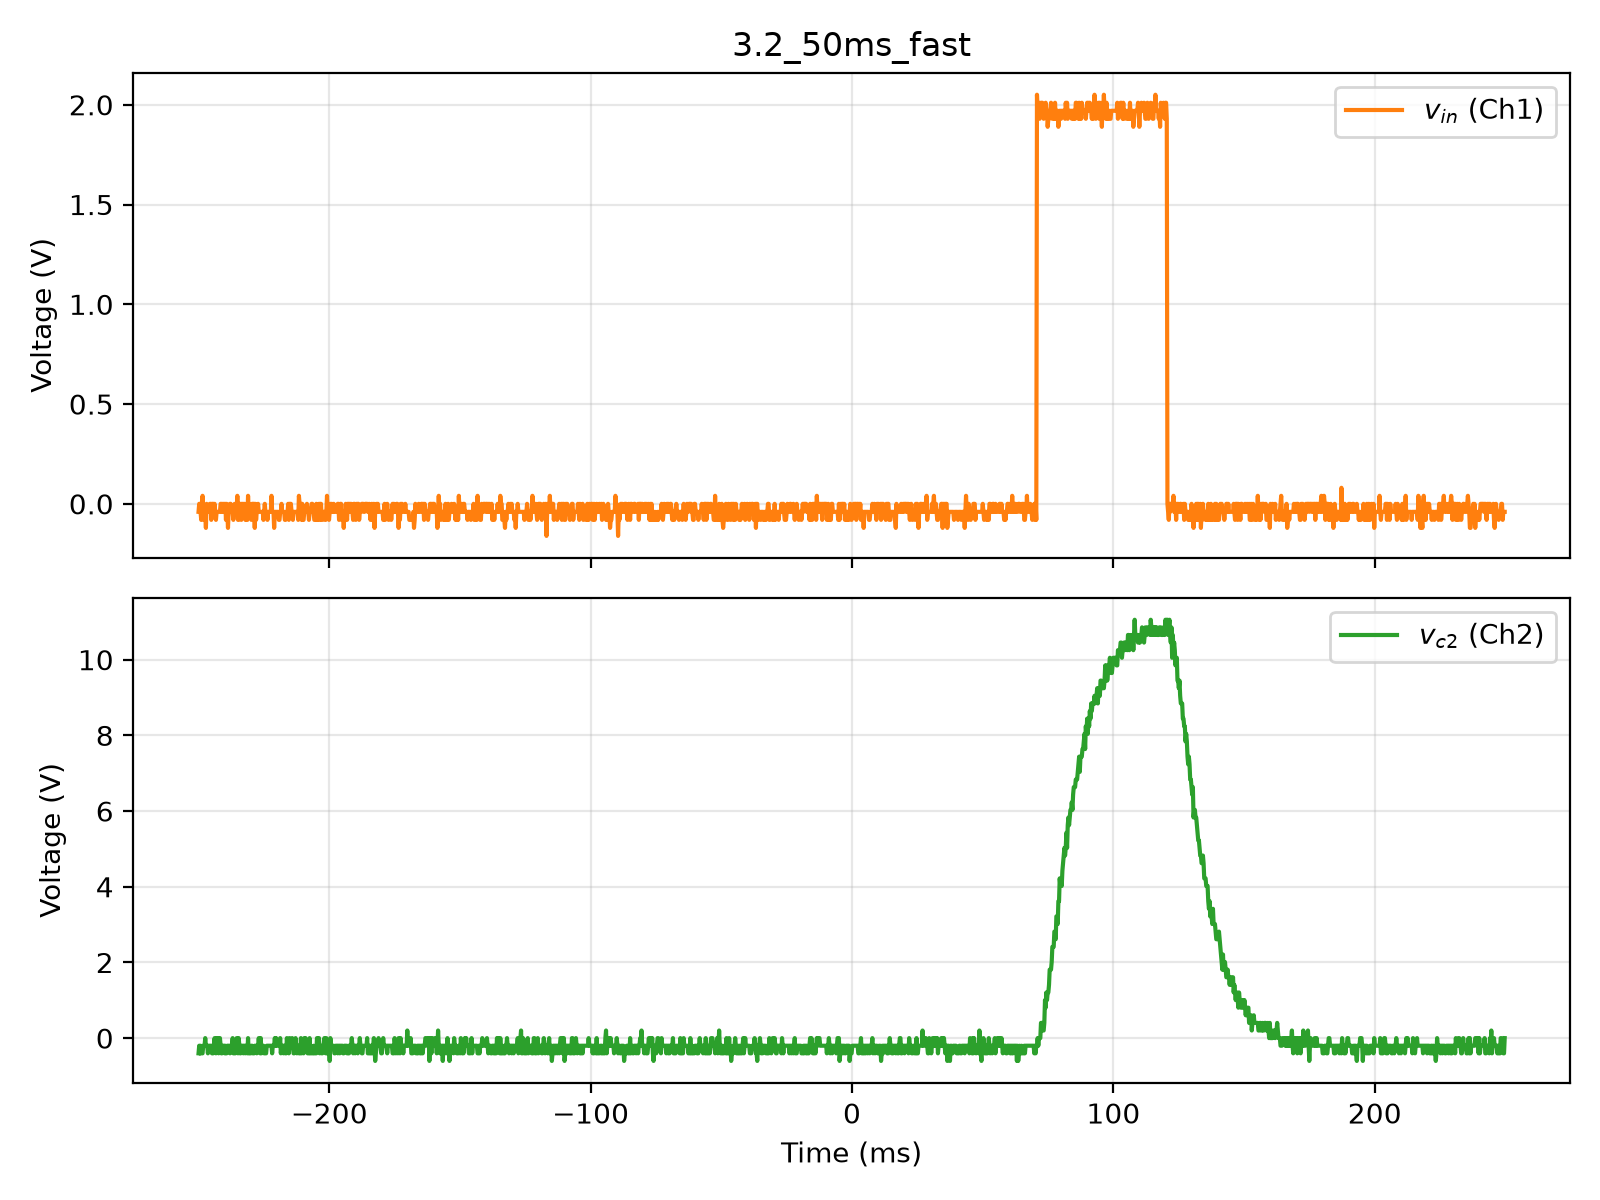
\includegraphics[width=0.48\textwidth]{3.2_50ms_fast.png}
    \caption{Slow and fast sweeps for the 50 ms pulse.}
    \label{fig:p50ms}
\end{figure}

\subsection*{Normalized traces vs.\ $h(t)$}
\addcontentsline{toc}{subsection}{Normalized traces}
\begin{figure}[H]
    \centering
 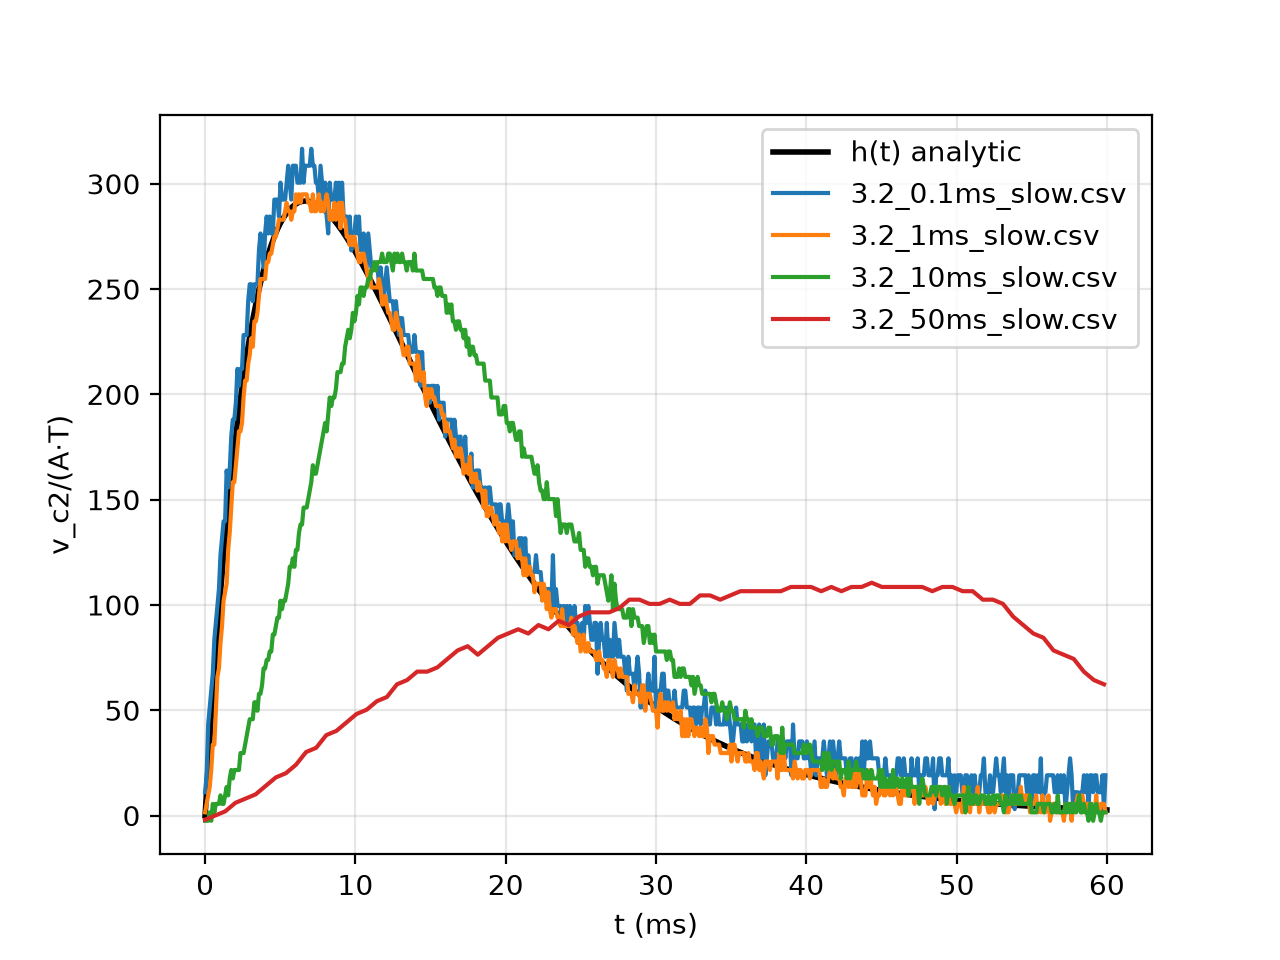
\includegraphics[width=0.9\textwidth]{3.2_normalized.png}
    \caption{Four measured $v_{c2}(t)$ traces normalized by pulse area, with analytic $h(t)$.}
    \label{fig:meas_norm}
\end{figure}
\textbf{Agreement with h(t):} The 100us and the 1ms have the best agreement with h(t), the peaks and timing of the other graphs don't line up nearly as well and this is due to the signal not acting like an impulse at the higher widths, so the circuit has time to respond. Errors on top of this point to component tolerances, oscilloscope measurements, and a non-ideal pulse from the function generator.

%---------------------------------------------------------------------
\newpage
\section*{Task 3.3: Step Response Measurements}
\addcontentsline{toc}{section}{Task 3.3}

\begin{figure}[H]
    \centering
     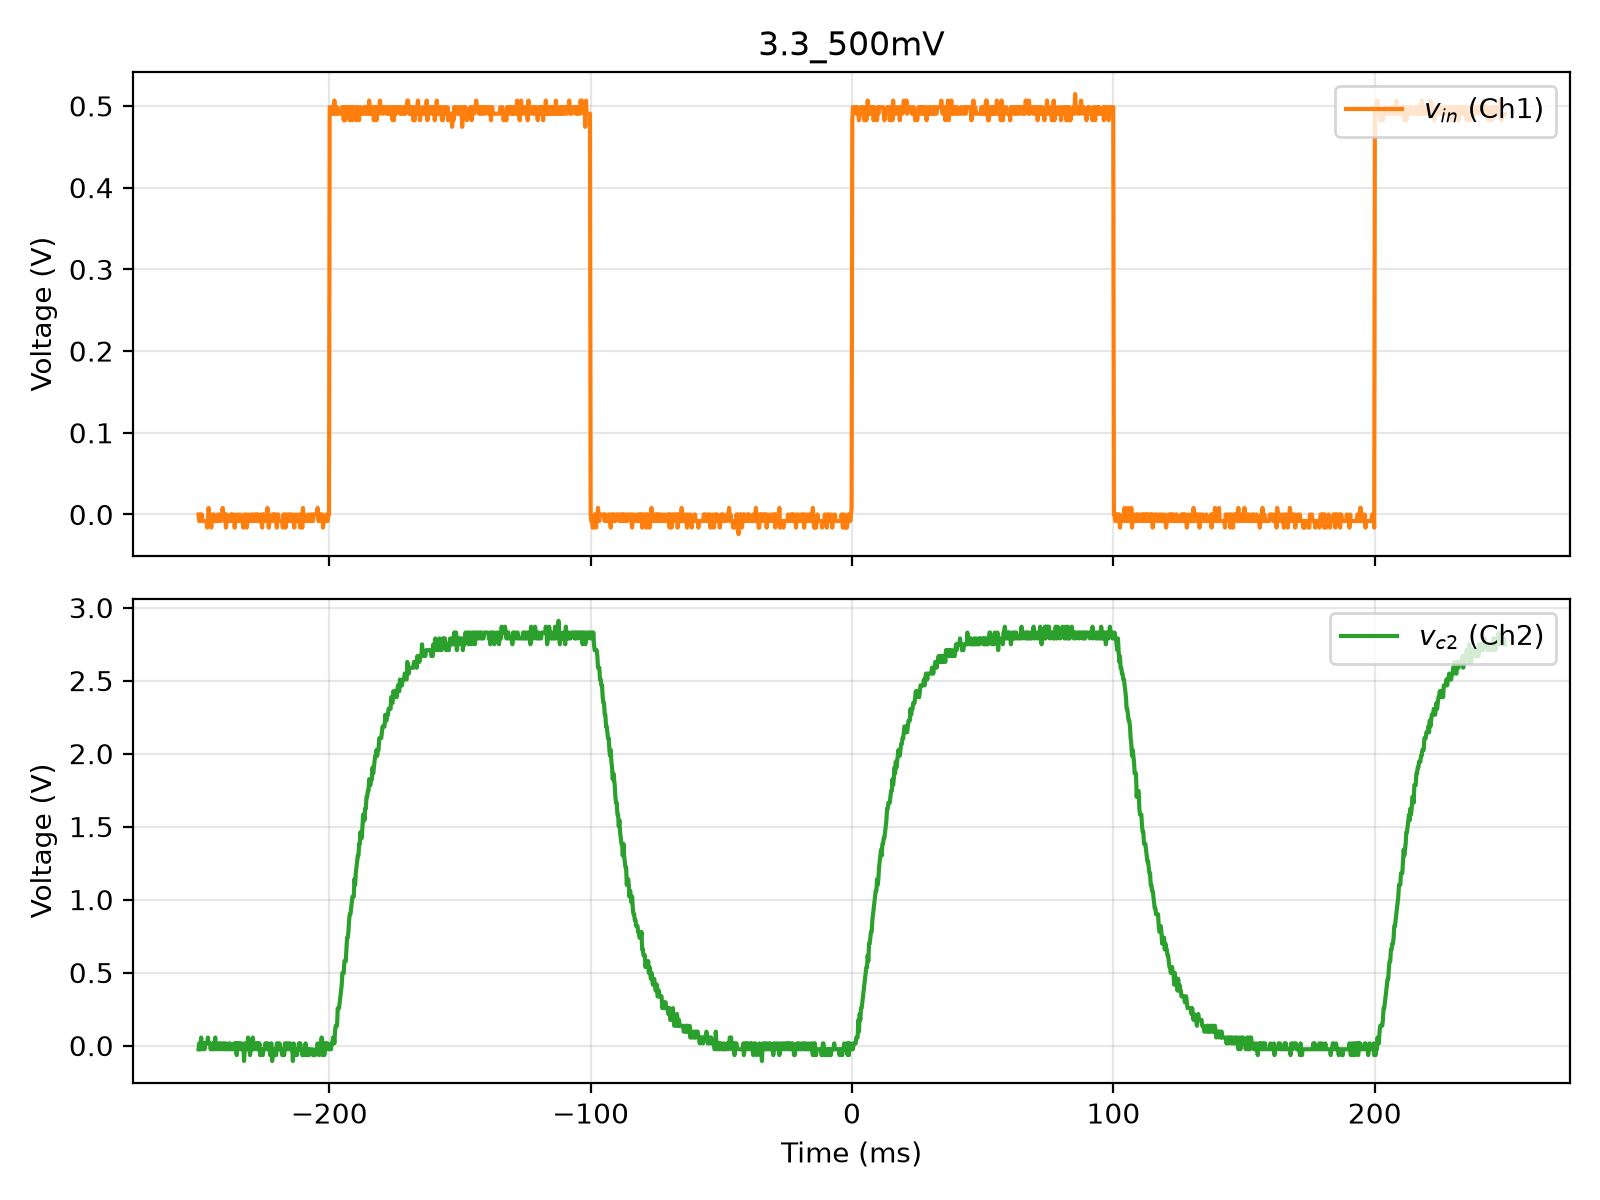
\includegraphics[width=0.9\textwidth]{3.3_500mV.png}
    \caption{Measured response to a 500 mV step (same rise and fall time constants).}
    \label{fig:step_500mV}
\end{figure}

\begin{figure}[H]
    \centering
    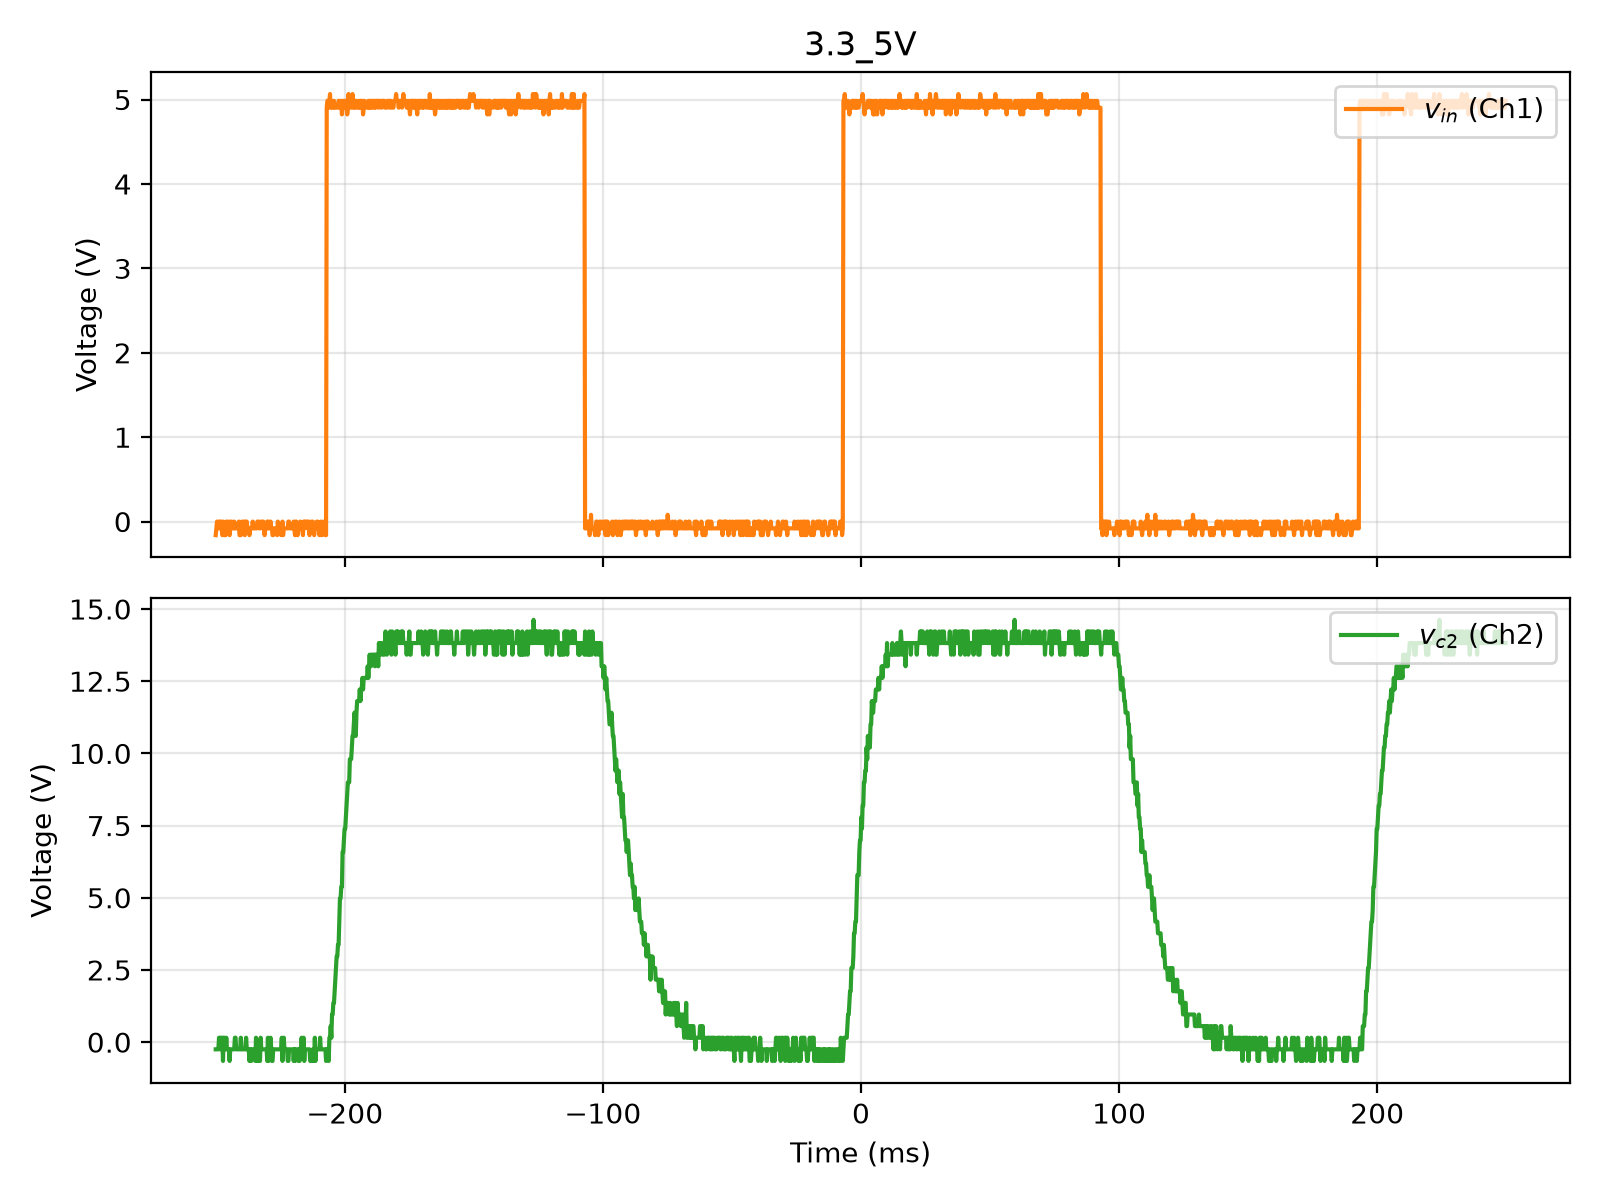
\includegraphics[width=0.9\textwidth]{3.3_5V.png}
    \caption{Measured response to a 5 V step (asymmetric rising/falling edges).}
    \label{fig:step_5V}
\end{figure}
The 500 mV step produced a smooth response with similar rise and fall behavior. The output reached about 0.7 V from a 0.5 V input, giving a measured gain of about 1.4. For the 5 V step, the output reached about 7.1 V and the rising and falling edges were no longer as similar. The output also appears to be limited near 7 V, also showing a gain of 1.42.

%---------------------------------------------------------------------
\newpage
\section*{Task 3.4: Frequency Response Measurements}
\addcontentsline{toc}{section}{Task 3.4}

\begin{table}[H]
    \centering
    \caption{Measured amplitude and time shift of $v_{c1}$ and $v_{c2}$.}
    \label{tab:freq}
    \begin{tabular}{c c c c c}
        \hline
        $f$ (Hz) & $V_{c1}$ (pp) & $\Delta t_1$ (ms) & $V_{c2}$ (pp) & $\Delta t_2$ (ms) \\
        \hline
        5   & 0.94 & 9.5 & 5.37 & 14.2 \\
        15  & 0.71 & 7.9 & 3.80 & 12.4 \\
        30  & 0.47   & 5.8  & 2.01 & 9.5  \\
        60  & 0.25 & 3.5 & 0.71 & 6.3  \\
        120 & 0.13 & 1.9 & 0.20 & 3.6  \\
        \hline
    \end{tabular}
\end{table}

\begin{figure}[H]
    \centering
     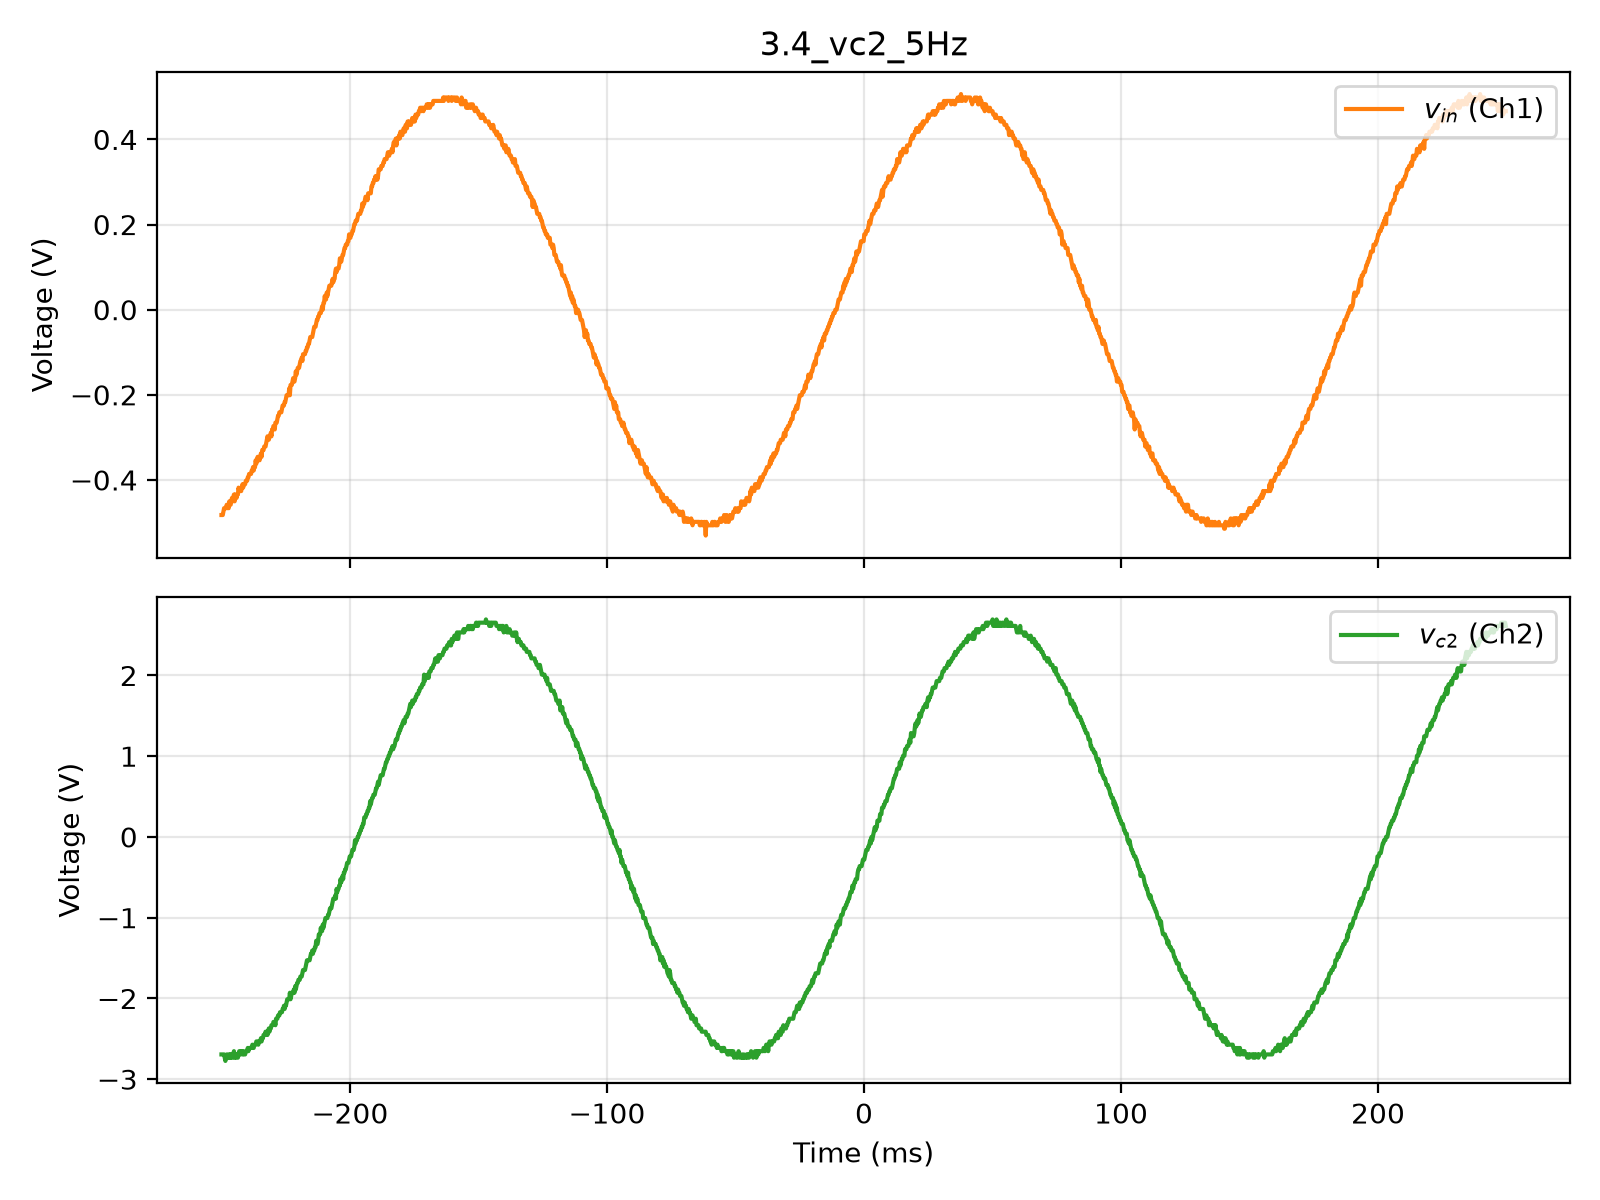
\includegraphics[width=0.9\textwidth]{3.4_vc2_5Hz.png}
    \caption{Measured $v_{c2}$ response to a 5 Hz sinusoidal input.}
    \label{}
\end{figure}
\begin{figure}[H]
    \centering
     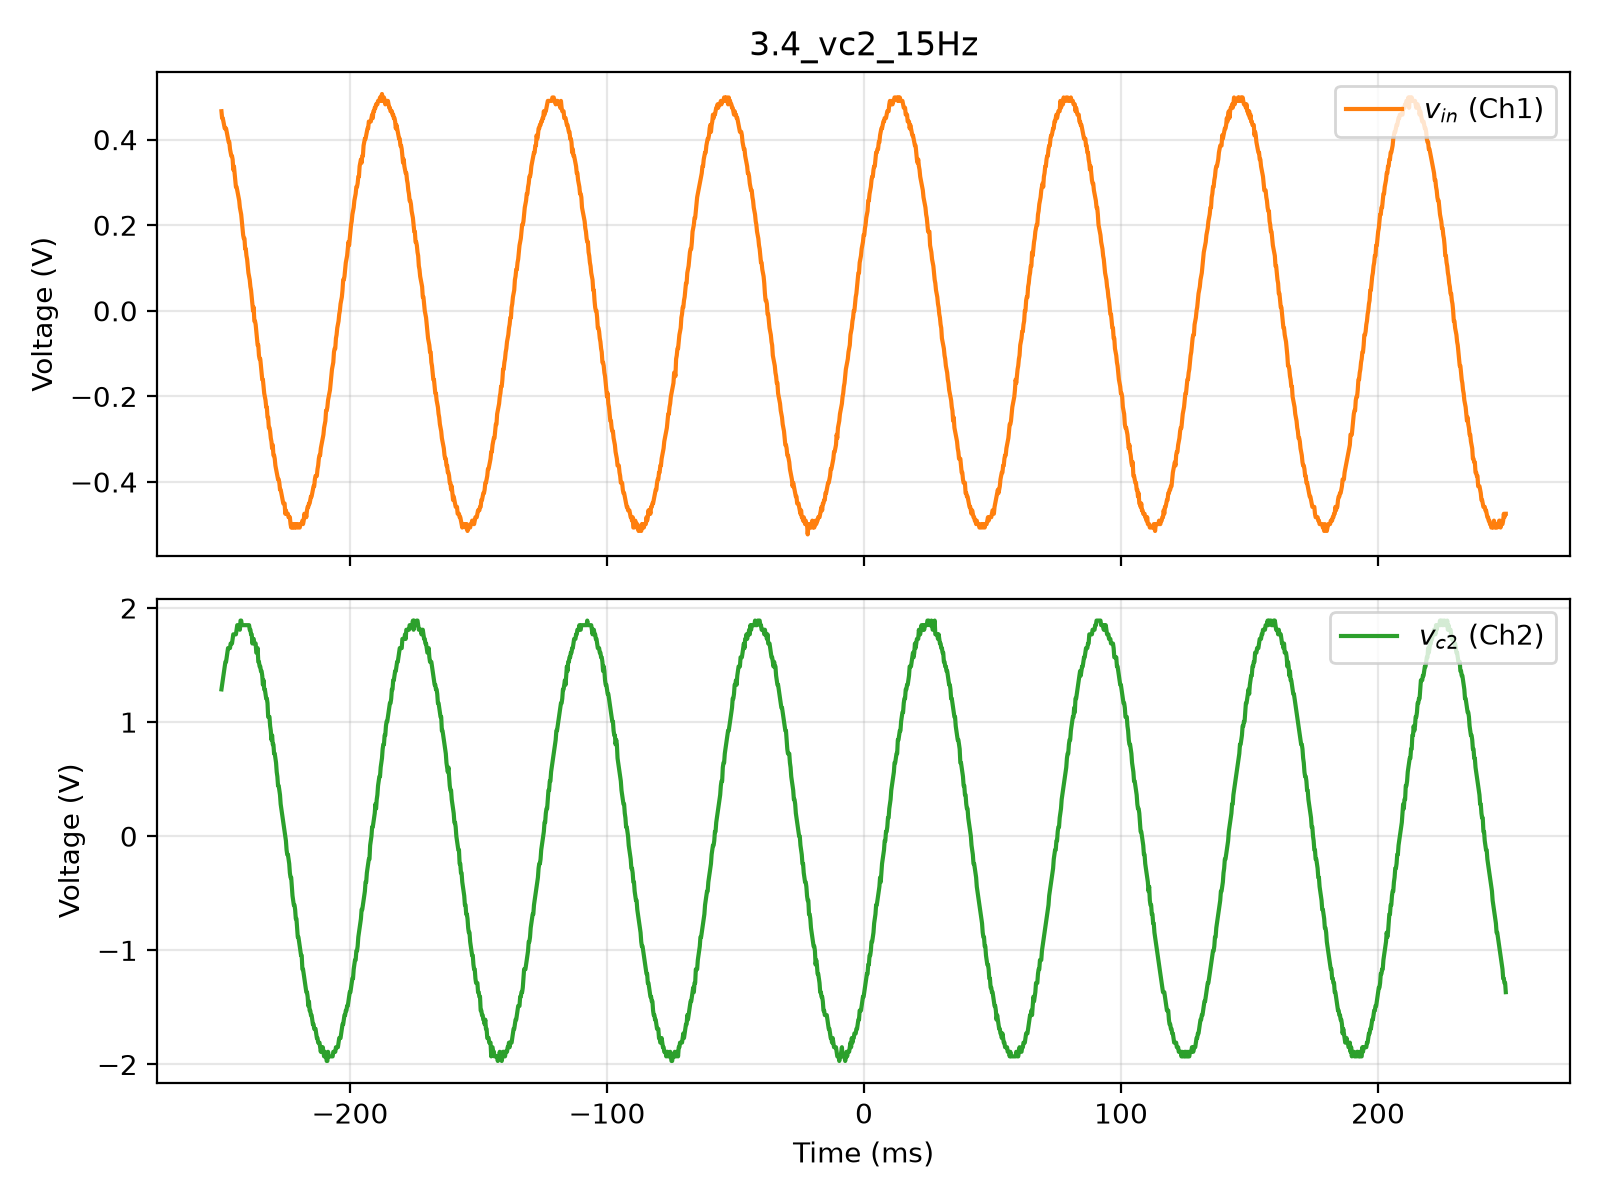
\includegraphics[width=0.9\textwidth]{3.4_vc2_15Hz.png}
   \caption{Measured $v_{c2}$ response to a 15 Hz sinusoidal input.}
    \label{}
\end{figure}
\begin{figure}[H]
    \centering
     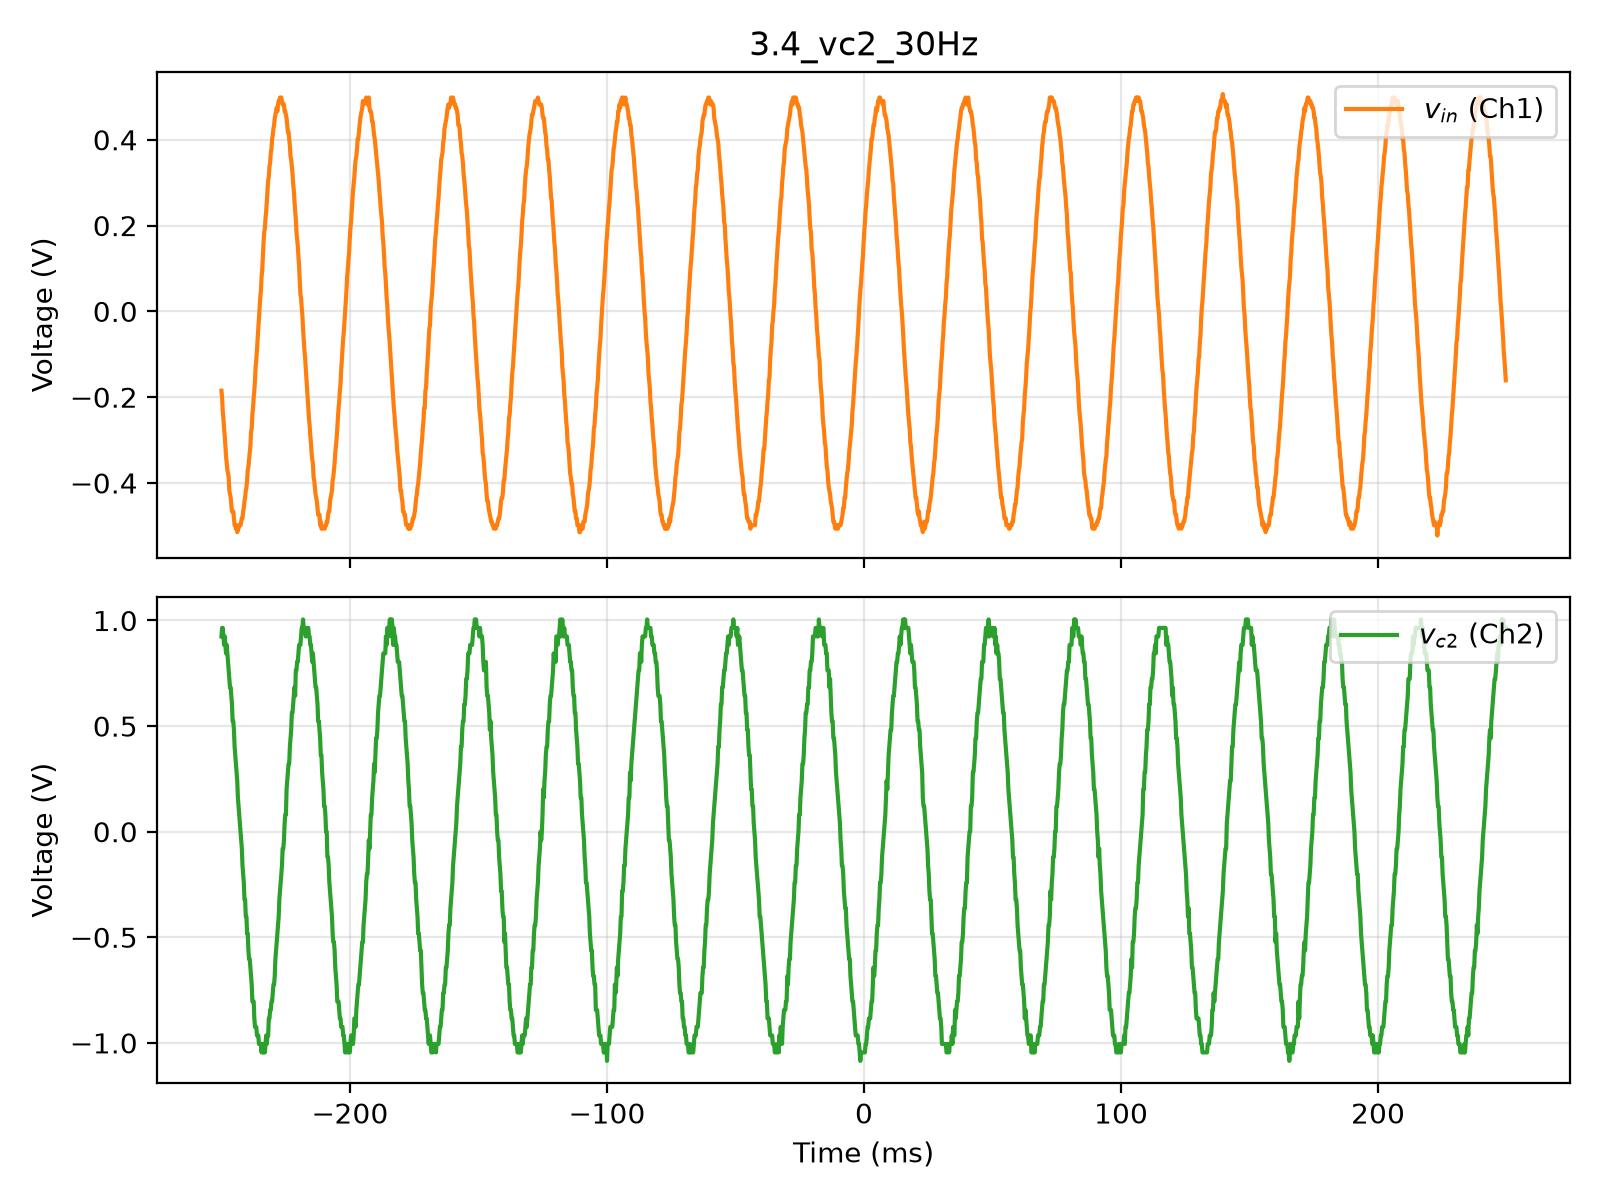
\includegraphics[width=0.9\textwidth]{3.4_vc2_30Hz.png}
   \caption{Measured $v_{c2}$ response to a 30 Hz sinusoidal input.}
    \label{}
\end{figure}

\begin{figure}[H]
    \centering
     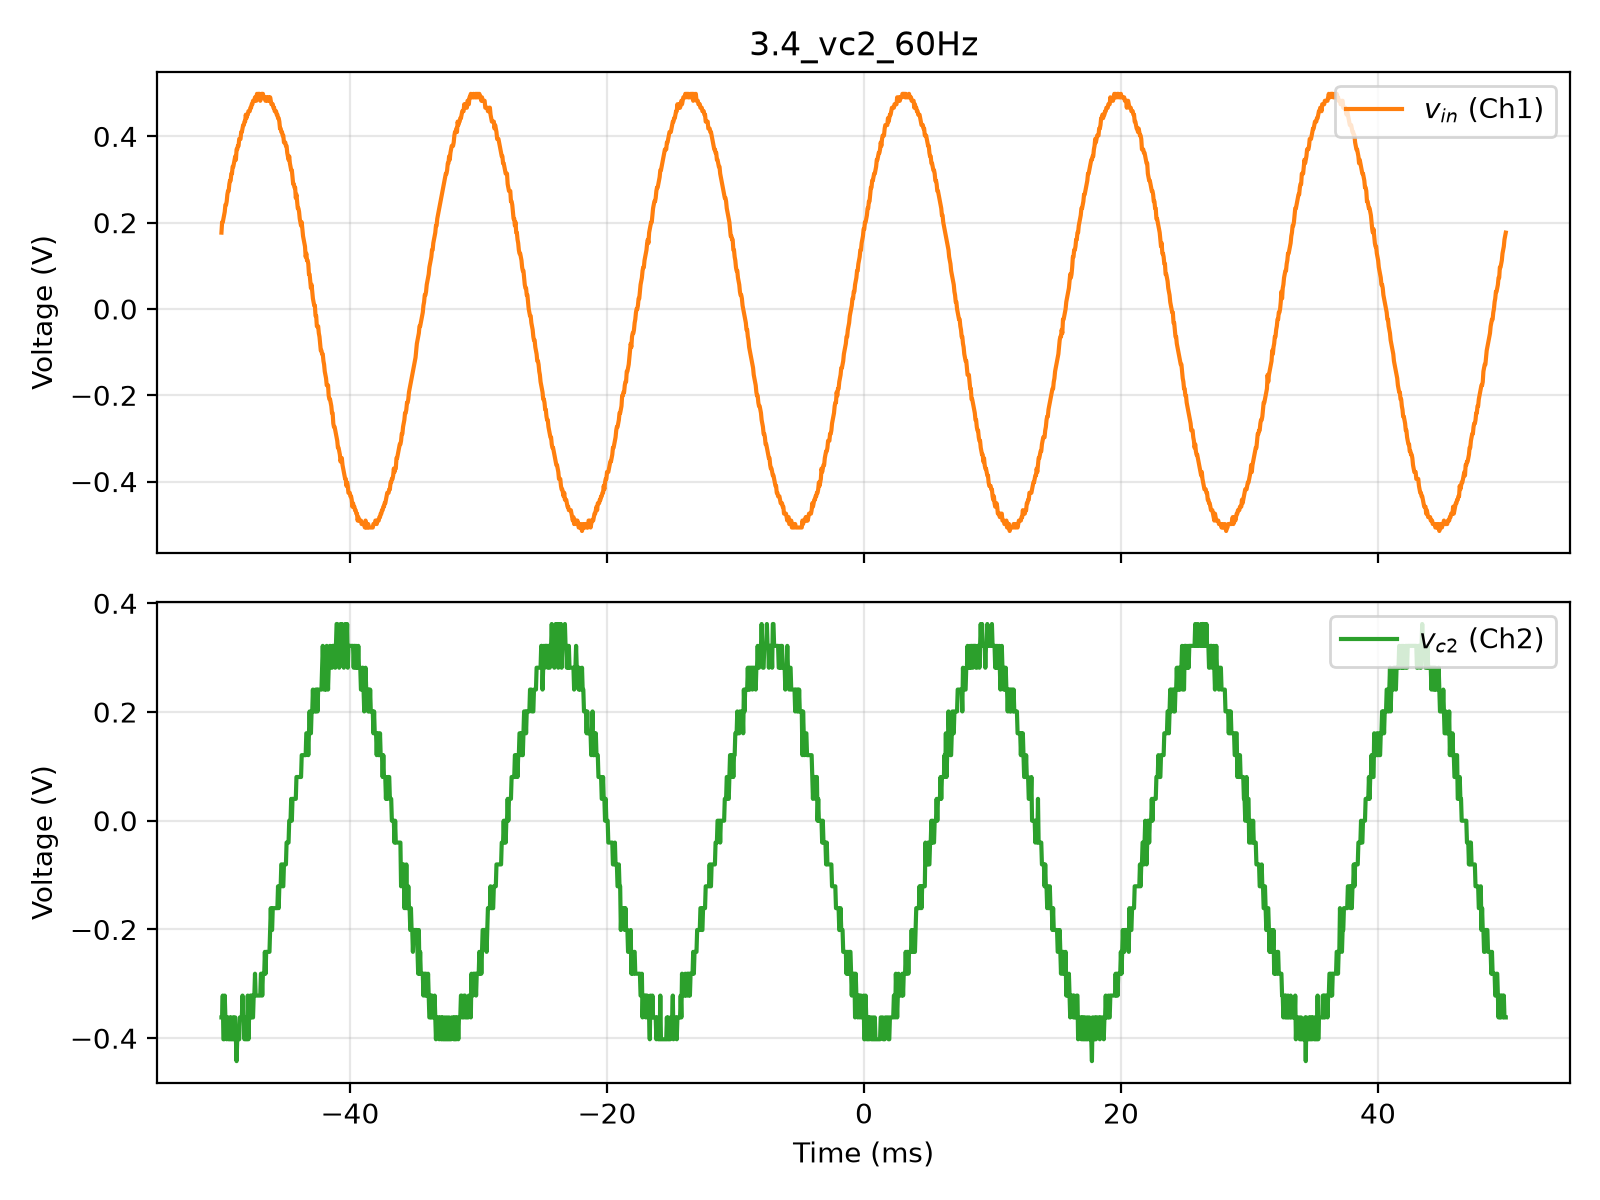
\includegraphics[width=0.9\textwidth]{3.4_vc2_60Hz.png}
\caption{Measured $v_{c2}$ response to a 60 Hz sinusoidal input.}
    \label{}
\end{figure}

\begin{figure}[H]
    \centering
     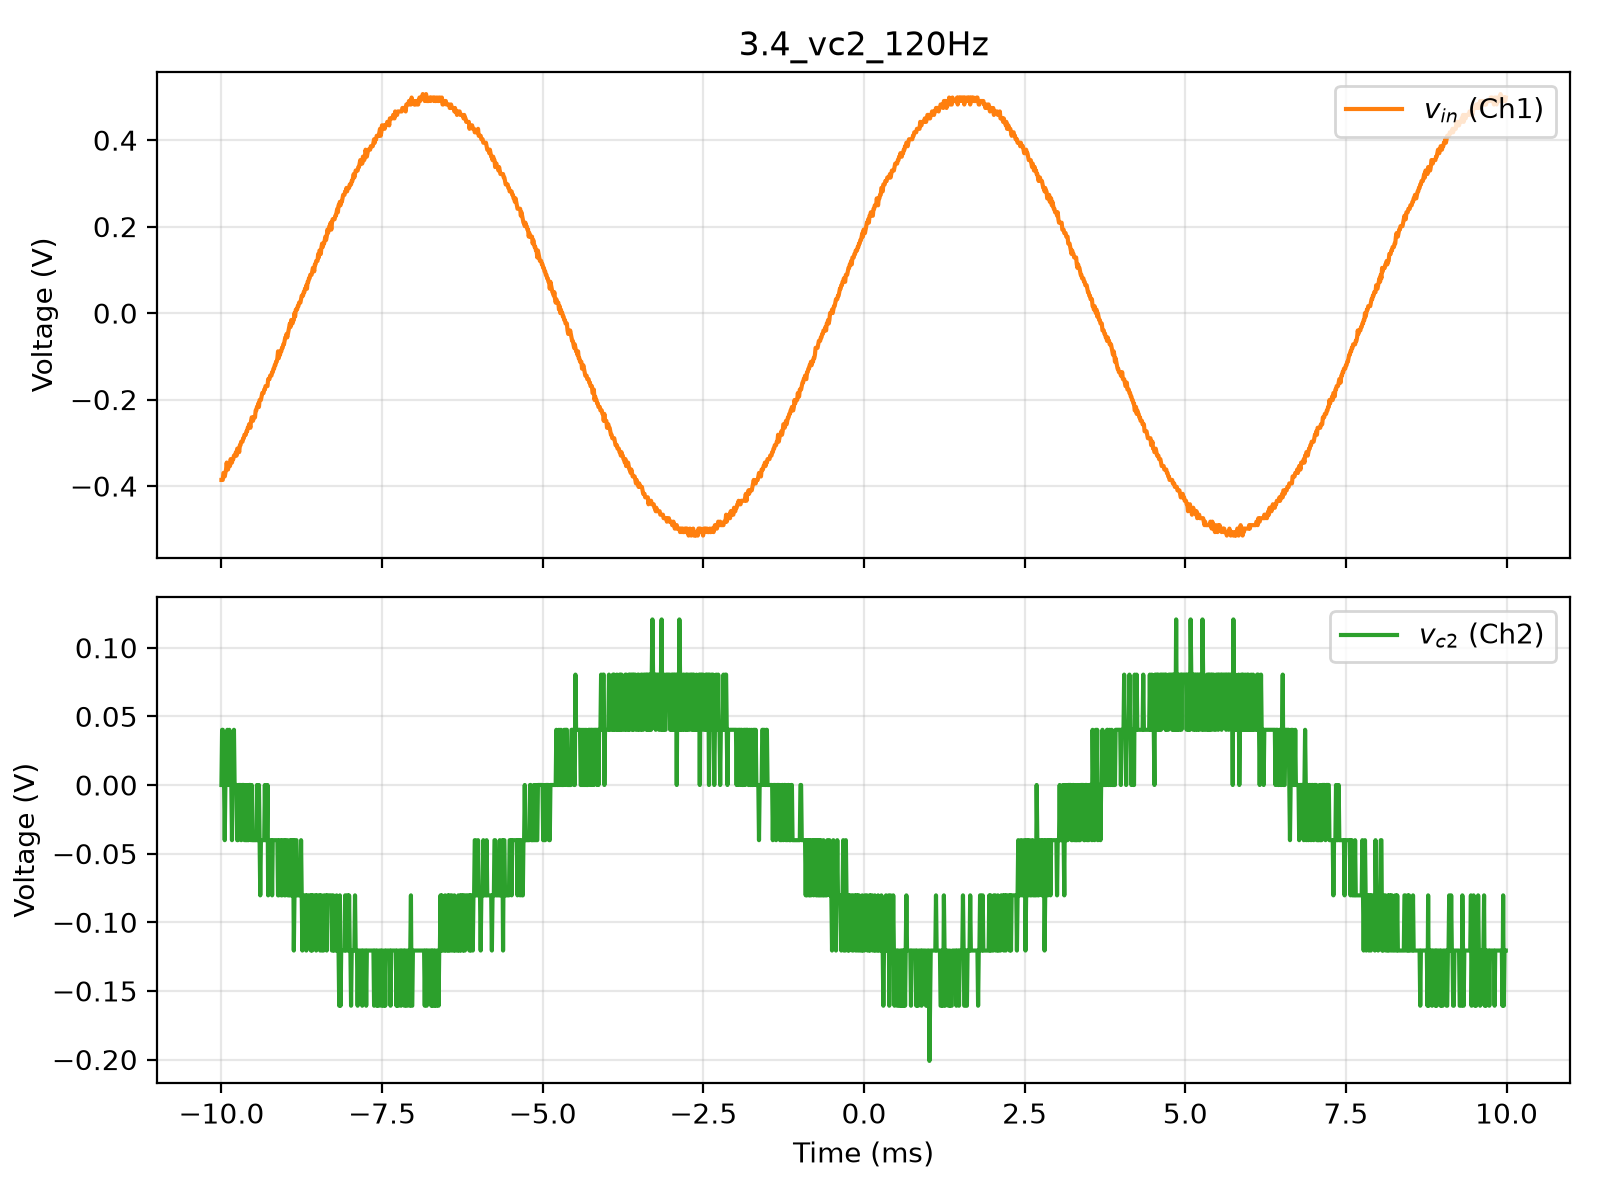
\includegraphics[width=0.9\textwidth]{3.4_vc2_120Hz.png}
    \caption{Measured $v_{c2}$ response to a 120 Hz sinusoidal input.}
    \label{}
\end{figure}


\begin{figure}[H]
    \centering
    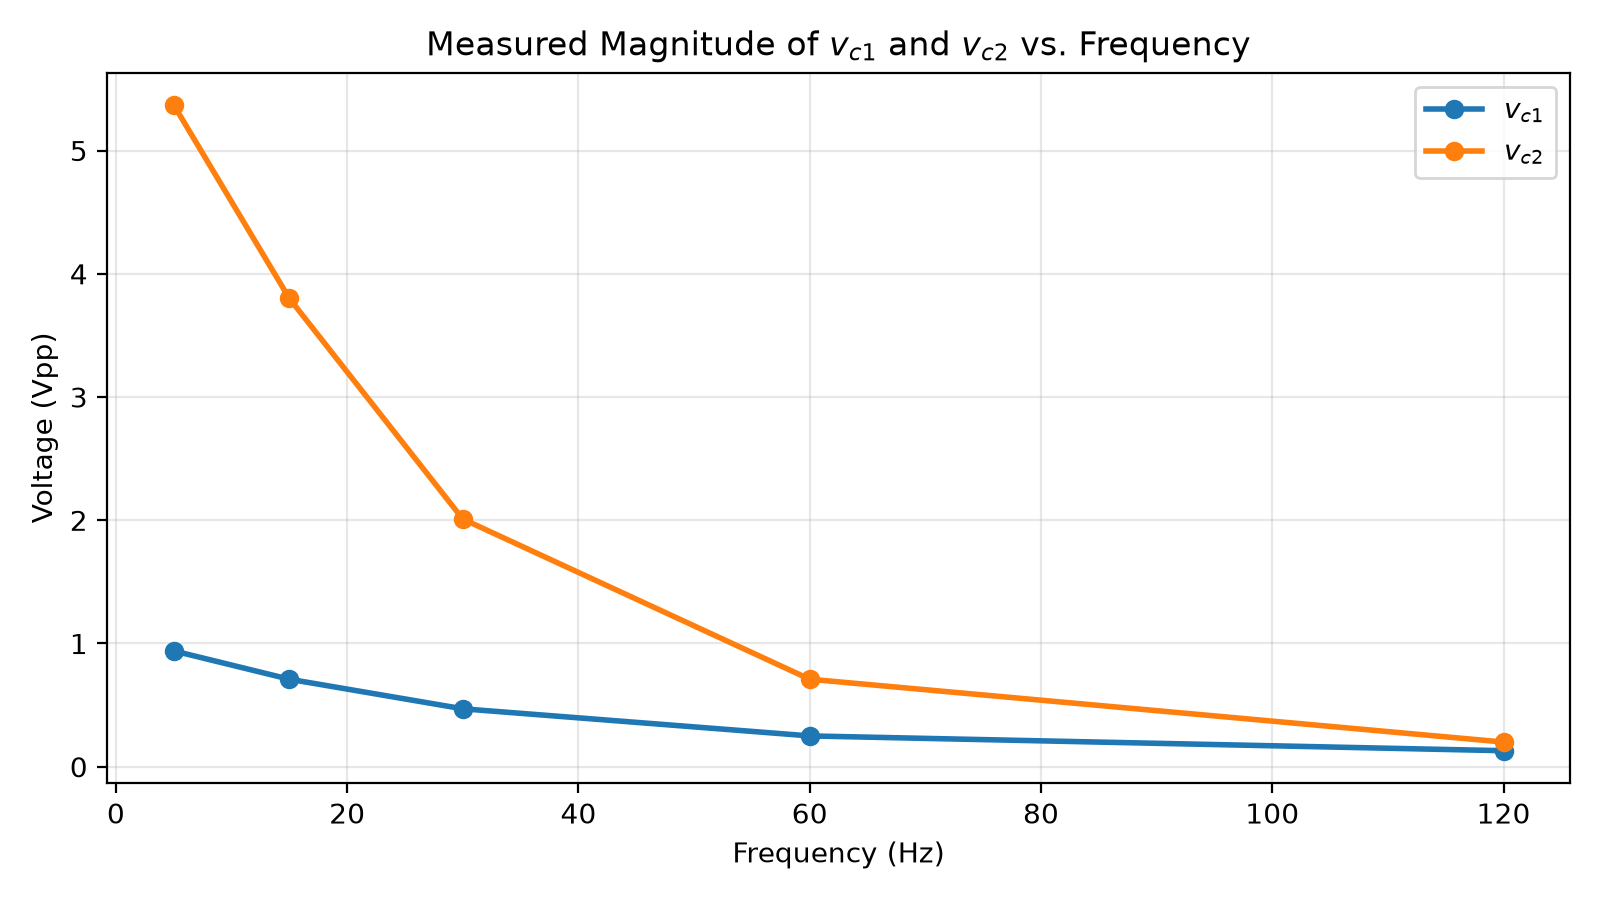
\includegraphics[width=0.8\textwidth]{task3_4_frequency_response.png}
    \caption{Measured magnitude of $v_{c1}$ and $v_{c2}$ versus frequency.}
    \label{fig:freq_mag}
\end{figure}
$V_{c2}$ Has a much larger roll off going from the same frequency it drops fro, 5.37 to .2, and $V_{c1}$ goes from .94 to .13V which is far slower roll off at least relative to $V_{c1}$.

%---------------------------------------------------------------------
\newpage
\section*{Conclusion}
\addcontentsline{toc}{section}{Conclusion}
% Summary of results per part (analysis, simulation, measurement), then takeaways:
% - linearity (amplitude scaling)
% - area matters, not shape, as T -> 0
% - T vs. tau_min rule
% - simulation vs. measurement agreement, sources of error

\newpage
\section*{Appendix}
\addcontentsline{toc}{section}{Appendix}
\subsection*{Task 3 Code}
\begin{lstlisting}[style=python, caption={Graphing raw CSVs and Table data for}]
import glob, os
import pandas as pd
import matplotlib
matplotlib.use("Agg")
import matplotlib.pyplot as plt

FOLDER = os.path.dirname(os.path.abspath(__file__))   # put this script in the CSV folder
OUT = os.path.join(FOLDER, "graphs")   # separate folder so scope .png files never get overwritten
os.makedirs(OUT, exist_ok=True)

for path in sorted(glob.glob(os.path.join(FOLDER, "*.csv"))):
    name = os.path.splitext(os.path.basename(path))[0]

    # skip the scope header, data starts at the  line
    with open(path, encoding="utf-8-sig") as f:
        skip = next(i for i, line in enumerate(f) if line.startswith("Sample Number"))
    df = pd.read_csv(path, skiprows=skip, encoding="utf-8-sig").dropna(axis=1, how="all")

    t = df["Time (s)"] * 1e3      # ms
    ch2 = r"$v_{c1}$" if "vc1" in name else r"$v_{c2}$"

    fig, ax = plt.subplots(figsize=(8, 4.5))
    ax.plot(t, df.iloc[:, 2], label=r"$v_{in}$ (Ch1)")
    ax.plot(t, df.iloc[:, 3], label=f"{ch2} (Ch2)")
    ax.set_xlabel("Time (ms)")
    ax.set_ylabel("Voltage (V)")
    ax.set_title(name)
    ax.grid(True, alpha=0.3)
    ax.legend(loc="upper right")
    fig.tight_layout()
    fig.savefig(os.path.join(OUT, name + ".png"), dpi=200)
    plt.close(fig)
    print("saved", name)


# Task 3.4 frequency response plot
frequency = [5, 15, 30, 60, 120]
vc1 = [0.94, 0.71, 0.47, 0.25, 0.13]
vc2 = [5.37, 3.80, 2.01, 0.71, 0.20]

fig, ax = plt.subplots(figsize=(8, 4.5))

ax.plot(frequency, vc1, marker="o", linewidth=2, label=r"$v_{c1}$")
ax.plot(frequency, vc2, marker="o", linewidth=2, label=r"$v_{c2}$")

ax.set_xlabel("Frequency (Hz)")
ax.set_ylabel("Voltage (Vpp)")
ax.set_title("Measured Magnitude of $v_{c1}$ and $v_{c2}$ vs. Frequency")
ax.grid(True, alpha=0.3)
ax.legend()

fig.tight_layout()
fig.savefig(os.path.join(OUT, "task3_4_frequency_response.png"), dpi=200)
plt.close(fig)



\end{lstlisting}

\newpage
\begin{lstlisting}[style=python, caption={Normalized Graph}]
import glob, os
import pandas as pd
import matplotlib
matplotlib.use("Agg")
import matplotlib.pyplot as plt

FOLDER = os.path.dirname(os.path.abspath(__file__))   # put this script in the CSV folder
OUT = os.path.join(FOLDER, "graphs")   # separate folder so scope .png files never get overwritten
os.makedirs(OUT, exist_ok=True)

for path in sorted(glob.glob(os.path.join(FOLDER, "*.csv"))):
    name = os.path.splitext(os.path.basename(path))[0]

    # skip the scope header, data starts at the  line
    with open(path, encoding="utf-8-sig") as f:
        skip = next(i for i, line in enumerate(f) if line.startswith("Sample Number"))
    df = pd.read_csv(path, skiprows=skip, encoding="utf-8-sig").dropna(axis=1, how="all")

    t = df["Time (s)"] * 1e3      # ms
    ch2 = r"$v_{c1}$" if "vc1" in name else r"$v_{c2}$"

    fig, ax = plt.subplots(figsize=(8, 4.5))
    ax.plot(t, df.iloc[:, 2], label=r"$v_{in}$ (Ch1)")
    ax.plot(t, df.iloc[:, 3], label=f"{ch2} (Ch2)")
    ax.set_xlabel("Time (ms)")
    ax.set_ylabel("Voltage (V)")
    ax.set_title(name)
    ax.grid(True, alpha=0.3)
    ax.legend(loc="upper right")
    fig.tight_layout()
    fig.savefig(os.path.join(OUT, name + ".png"), dpi=200)
    plt.close(fig)
    print("saved", name)



\end{lstlisting}

\end{document}